\documentclass[aspectratio=169,10pt]{beamer}
\usepackage[T1]{fontenc}
\usepackage[scaled=0.9]{helvet}   % stand-in for Amazon Ember (not installed)
\renewcommand{\familydefault}{\sfdefault}
\usepackage{booktabs,tabularx,multirow,makecell,colortbl,xcolor}
\usepackage{graphicx}
\usepackage{pgfplots}
\pgfplotsset{compat=1.18}
\usepackage{listings}
\usepackage{fontawesome5}

% ---- AWS template palette (dark) ----------------------------------
\definecolor{bgdark}{HTML}{161D26}
\definecolor{panel}{HTML}{232F3E}
\definecolor{awsblue}{HTML}{007DFF}
\definecolor{awspurple}{HTML}{952EFF}
\definecolor{awsmagenta}{HTML}{E433FF}
\definecolor{awsteal}{HTML}{00D6C7}
\definecolor{bodytext}{HTML}{F2F4F7}
\definecolor{inkmuted}{HTML}{A3ACB9}
\definecolor{footc}{HTML}{8B95A3}
\definecolor{rulec}{HTML}{5A6573}
\definecolor{gridc}{HTML}{333E4C}
\definecolor{vendorc}{HTML}{7B8594}
\definecolor{linkc}{HTML}{5FB0FF}
\definecolor{sectag}{HTML}{E433FF}
% extra categorical colours for charts, tuned for the dark background
\definecolor{cat1}{HTML}{EB6834}   % orange
\definecolor{cat2}{HTML}{3B8BEB}   % blue
\definecolor{cat3}{HTML}{1BAF7A}   % aqua

% footer text; override with \renewcommand{\deckfooter}{...} after \documentclass[aspectratio=169,10pt]{beamer}
\usepackage[T1]{fontenc}
\usepackage[scaled=0.9]{helvet}   % stand-in for Amazon Ember (not installed)
\renewcommand{\familydefault}{\sfdefault}
\usepackage{booktabs,tabularx,multirow,makecell,colortbl,xcolor}
\usepackage{graphicx}
\usepackage{pgfplots}
\pgfplotsset{compat=1.18}
\usepackage{listings}
\usepackage{fontawesome5}

% ---- AWS template palette (dark) ----------------------------------
\definecolor{bgdark}{HTML}{161D26}
\definecolor{panel}{HTML}{232F3E}
\definecolor{awsblue}{HTML}{007DFF}
\definecolor{awspurple}{HTML}{952EFF}
\definecolor{awsmagenta}{HTML}{E433FF}
\definecolor{awsteal}{HTML}{00D6C7}
\definecolor{bodytext}{HTML}{F2F4F7}
\definecolor{inkmuted}{HTML}{A3ACB9}
\definecolor{footc}{HTML}{8B95A3}
\definecolor{rulec}{HTML}{5A6573}
\definecolor{gridc}{HTML}{333E4C}
\definecolor{vendorc}{HTML}{7B8594}
\definecolor{linkc}{HTML}{5FB0FF}
\definecolor{sectag}{HTML}{E433FF}
% extra categorical colours for charts, tuned for the dark background
\definecolor{cat1}{HTML}{EB6834}   % orange
\definecolor{cat2}{HTML}{3B8BEB}   % blue
\definecolor{cat3}{HTML}{1BAF7A}   % aqua

% footer text; override with \renewcommand{\deckfooter}{...} after \documentclass[aspectratio=169,10pt]{beamer}
\usepackage[T1]{fontenc}
\usepackage[scaled=0.9]{helvet}   % stand-in for Amazon Ember (not installed)
\renewcommand{\familydefault}{\sfdefault}
\usepackage{booktabs,tabularx,multirow,makecell,colortbl,xcolor}
\usepackage{graphicx}
\usepackage{pgfplots}
\pgfplotsset{compat=1.18}
\usepackage{listings}
\usepackage{fontawesome5}

% ---- AWS template palette (dark) ----------------------------------
\definecolor{bgdark}{HTML}{161D26}
\definecolor{panel}{HTML}{232F3E}
\definecolor{awsblue}{HTML}{007DFF}
\definecolor{awspurple}{HTML}{952EFF}
\definecolor{awsmagenta}{HTML}{E433FF}
\definecolor{awsteal}{HTML}{00D6C7}
\definecolor{bodytext}{HTML}{F2F4F7}
\definecolor{inkmuted}{HTML}{A3ACB9}
\definecolor{footc}{HTML}{8B95A3}
\definecolor{rulec}{HTML}{5A6573}
\definecolor{gridc}{HTML}{333E4C}
\definecolor{vendorc}{HTML}{7B8594}
\definecolor{linkc}{HTML}{5FB0FF}
\definecolor{sectag}{HTML}{E433FF}
% extra categorical colours for charts, tuned for the dark background
\definecolor{cat1}{HTML}{EB6834}   % orange
\definecolor{cat2}{HTML}{3B8BEB}   % blue
\definecolor{cat3}{HTML}{1BAF7A}   % aqua

% footer text; override with \renewcommand{\deckfooter}{...} after \input{preamble}
\newcommand{\deckfooter}{\textcopyright{} \the\year, Amazon Web Services, Inc. or its affiliates.}

% ---- beamer look ---------------------------------------------------
\setbeamercolor{background canvas}{bg=bgdark}
\setbeamercolor{normal text}{fg=bodytext,bg=bgdark}
\setbeamercolor{structure}{fg=awsblue}
\setbeamercolor{frametitle}{fg=white}
\setbeamercolor{itemize item}{fg=awsteal}
\setbeamercolor{itemize subitem}{fg=inkmuted}
\setbeamercolor{enumerate item}{fg=awsteal}
\setbeamercolor{alerted text}{fg=awsmagenta}
\setbeamertemplate{navigation symbols}{}
\setbeamertemplate{itemize items}[square]
\setbeamertemplate{enumerate items}[default]
\setbeamertemplate{caption}[numbered]
\setbeamerfont{itemize/enumerate subbody}{size=\scriptsize}
\setbeamersize{text margin left=8mm,text margin right=8mm}

% section tag shown above each frame title (no divider slides)
\gdef\secname{}
\newcommand{\sect}[1]{\section{#1}\gdef\secname{#1}}
\setbeamertemplate{frametitle}{%
  \nointerlineskip\vskip3.2mm
  \ifx\secname\empty\else{\fontsize{6.5}{7}\selectfont\bfseries\color{sectag}\MakeUppercase{\secname}}\par\vskip0.9mm\fi
  {\fontsize{12.5}{14.5}\selectfont\bfseries\color{white}\insertframetitle}\par\vskip0.6mm}
\setbeamertemplate{headline}{}
\setbeamertemplate{footline}{%
  \hbox to\paperwidth{\hspace*{8mm}{\fontsize{5}{6}\selectfont\color{footc}\deckfooter}\hfill{\fontsize{6}{7}\selectfont\color{footc}\insertframenumber}\hspace*{8mm}}\vskip2.5mm}

% ---- deck macros ---------------------------------------------------
\newcommand{\hl}[1]{\textcolor{awsteal}{\textbf{#1}}}
\newcommand{\src}[1]{\vfill{\tiny\textcolor{footc}{Source: #1}}}
\newcommand{\flabel}[1]{\label{#1}\hypertarget{#1}{}}
% clickable slide references
\newcommand{\sref}[1]{\hyperlink{#1}{\textcolor{linkc}{slide~\pageref*{#1}}}}
\newcommand{\srefs}[2]{\textcolor{linkc}{slides~\hyperlink{#1}{\pageref*{#1}}--\hyperlink{#2}{\pageref*{#2}}}}
\newcommand{\plainen}[1]{\colorbox{panel}{\parbox{\dimexpr\linewidth-2\fboxsep}{\raggedright\footnotesize\textbf{In plain English:} #1}}\par\vspace{1mm}}
\newcommand{\idcard}[1]{\colorbox{panel}{\parbox{\dimexpr\textwidth-2\fboxsep}{\scriptsize #1}}}
\newcommand{\grp}[2]{\multicolumn{#1}{@{}l}{\textcolor{awsteal}{\textit{#2}}}}
\newcommand{\agi}[4]{\hyperlink{#1}{{\large\bfseries\color{awsteal}#2}\quad{\large\bfseries\color{white}#3}}\\[0.5mm]{\small\color{inkmuted}#4}\par\vspace{4mm}}
\newcommand{\bgframe}[1]{\usebackgroundtemplate{\includegraphics[width=\paperwidth,height=\paperheight]{#1}}}

\arrayrulecolor{rulec}
\lstset{basicstyle=\ttfamily\tiny\color{bodytext},breaklines=true,columns=fullflexible,
  backgroundcolor=\color{panel},frame=single,rulecolor=\color{rulec},
  keywordstyle=\color{awsteal}\bfseries,commentstyle=\color{inkmuted},showstringspaces=false}
\renewcommand{\arraystretch}{1.1}
\usetikzlibrary{arrows.meta,positioning,shapes.geometric,calc,fit,backgrounds,shadows}
\tikzset{box/.style={draw=awsblue,fill=panel,rounded corners=2pt,align=center,font=\scriptsize,inner sep=3pt,text=bodytext},
         arr/.style={-{Stealth[length=2mm]},thick,awsblue}}
\pgfplotsset{every axis/.append style={axis line style={rulec},tick style={rulec},
  tick label style={text=bodytext},label style={text=bodytext}}}

% numbered table / figure labels (one index across the deck)
\newcounter{tabno}\newcounter{figno}
\newcommand{\tabcap}[1]{\refstepcounter{tabno}{\scriptsize\bfseries\color{awsteal}Table~\thetabno\hspace{0.6em}{\color{bodytext}#1}}\par\vspace{0.2mm}}
\newcommand{\figcap}[1]{\refstepcounter{figno}{\scriptsize\bfseries\color{awsteal}Figure~\thefigno\hspace{0.6em}{\color{bodytext}#1}}\par\vspace{0.2mm}}

% ---- table helpers -------------------------------------------------
\newcommand{\tb}[1]{\texttt{#1}}
\newcolumntype{P}[1]{>{\raggedright\arraybackslash}p{#1}}
\newcolumntype{Y}{>{\raggedright\arraybackslash}X}
% substrate names in their fixed chart colours (blue / orange / aqua)
\newcommand{\smv}{\textcolor{cat2}{\textbf{microVM}}}
\newcommand{\sm}{\textcolor{cat1}{\textbf{m5}}}
\newcommand{\sg}{\textcolor{cat3}{\textbf{g6}}}

\newcommand{\deckfooter}{\textcopyright{} \the\year, Amazon Web Services, Inc. or its affiliates.}

% ---- beamer look ---------------------------------------------------
\setbeamercolor{background canvas}{bg=bgdark}
\setbeamercolor{normal text}{fg=bodytext,bg=bgdark}
\setbeamercolor{structure}{fg=awsblue}
\setbeamercolor{frametitle}{fg=white}
\setbeamercolor{itemize item}{fg=awsteal}
\setbeamercolor{itemize subitem}{fg=inkmuted}
\setbeamercolor{enumerate item}{fg=awsteal}
\setbeamercolor{alerted text}{fg=awsmagenta}
\setbeamertemplate{navigation symbols}{}
\setbeamertemplate{itemize items}[square]
\setbeamertemplate{enumerate items}[default]
\setbeamertemplate{caption}[numbered]
\setbeamerfont{itemize/enumerate subbody}{size=\scriptsize}
\setbeamersize{text margin left=8mm,text margin right=8mm}

% section tag shown above each frame title (no divider slides)
\gdef\secname{}
\newcommand{\sect}[1]{\section{#1}\gdef\secname{#1}}
\setbeamertemplate{frametitle}{%
  \nointerlineskip\vskip3.2mm
  \ifx\secname\empty\else{\fontsize{6.5}{7}\selectfont\bfseries\color{sectag}\MakeUppercase{\secname}}\par\vskip0.9mm\fi
  {\fontsize{12.5}{14.5}\selectfont\bfseries\color{white}\insertframetitle}\par\vskip0.6mm}
\setbeamertemplate{headline}{}
\setbeamertemplate{footline}{%
  \hbox to\paperwidth{\hspace*{8mm}{\fontsize{5}{6}\selectfont\color{footc}\deckfooter}\hfill{\fontsize{6}{7}\selectfont\color{footc}\insertframenumber}\hspace*{8mm}}\vskip2.5mm}

% ---- deck macros ---------------------------------------------------
\newcommand{\hl}[1]{\textcolor{awsteal}{\textbf{#1}}}
\newcommand{\src}[1]{\vfill{\tiny\textcolor{footc}{Source: #1}}}
\newcommand{\flabel}[1]{\label{#1}\hypertarget{#1}{}}
% clickable slide references
\newcommand{\sref}[1]{\hyperlink{#1}{\textcolor{linkc}{slide~\pageref*{#1}}}}
\newcommand{\srefs}[2]{\textcolor{linkc}{slides~\hyperlink{#1}{\pageref*{#1}}--\hyperlink{#2}{\pageref*{#2}}}}
\newcommand{\plainen}[1]{\colorbox{panel}{\parbox{\dimexpr\linewidth-2\fboxsep}{\raggedright\footnotesize\textbf{In plain English:} #1}}\par\vspace{1mm}}
\newcommand{\idcard}[1]{\colorbox{panel}{\parbox{\dimexpr\textwidth-2\fboxsep}{\scriptsize #1}}}
\newcommand{\grp}[2]{\multicolumn{#1}{@{}l}{\textcolor{awsteal}{\textit{#2}}}}
\newcommand{\agi}[4]{\hyperlink{#1}{{\large\bfseries\color{awsteal}#2}\quad{\large\bfseries\color{white}#3}}\\[0.5mm]{\small\color{inkmuted}#4}\par\vspace{4mm}}
\newcommand{\bgframe}[1]{\usebackgroundtemplate{\includegraphics[width=\paperwidth,height=\paperheight]{#1}}}

\arrayrulecolor{rulec}
\lstset{basicstyle=\ttfamily\tiny\color{bodytext},breaklines=true,columns=fullflexible,
  backgroundcolor=\color{panel},frame=single,rulecolor=\color{rulec},
  keywordstyle=\color{awsteal}\bfseries,commentstyle=\color{inkmuted},showstringspaces=false}
\renewcommand{\arraystretch}{1.1}
\usetikzlibrary{arrows.meta,positioning,shapes.geometric,calc,fit,backgrounds,shadows}
\tikzset{box/.style={draw=awsblue,fill=panel,rounded corners=2pt,align=center,font=\scriptsize,inner sep=3pt,text=bodytext},
         arr/.style={-{Stealth[length=2mm]},thick,awsblue}}
\pgfplotsset{every axis/.append style={axis line style={rulec},tick style={rulec},
  tick label style={text=bodytext},label style={text=bodytext}}}

% numbered table / figure labels (one index across the deck)
\newcounter{tabno}\newcounter{figno}
\newcommand{\tabcap}[1]{\refstepcounter{tabno}{\scriptsize\bfseries\color{awsteal}Table~\thetabno\hspace{0.6em}{\color{bodytext}#1}}\par\vspace{0.2mm}}
\newcommand{\figcap}[1]{\refstepcounter{figno}{\scriptsize\bfseries\color{awsteal}Figure~\thefigno\hspace{0.6em}{\color{bodytext}#1}}\par\vspace{0.2mm}}

% ---- table helpers -------------------------------------------------
\newcommand{\tb}[1]{\texttt{#1}}
\newcolumntype{P}[1]{>{\raggedright\arraybackslash}p{#1}}
\newcolumntype{Y}{>{\raggedright\arraybackslash}X}
% substrate names in their fixed chart colours (blue / orange / aqua)
\newcommand{\smv}{\textcolor{cat2}{\textbf{microVM}}}
\newcommand{\sm}{\textcolor{cat1}{\textbf{m5}}}
\newcommand{\sg}{\textcolor{cat3}{\textbf{g6}}}

\newcommand{\deckfooter}{\textcopyright{} \the\year, Amazon Web Services, Inc. or its affiliates.}

% ---- beamer look ---------------------------------------------------
\setbeamercolor{background canvas}{bg=bgdark}
\setbeamercolor{normal text}{fg=bodytext,bg=bgdark}
\setbeamercolor{structure}{fg=awsblue}
\setbeamercolor{frametitle}{fg=white}
\setbeamercolor{itemize item}{fg=awsteal}
\setbeamercolor{itemize subitem}{fg=inkmuted}
\setbeamercolor{enumerate item}{fg=awsteal}
\setbeamercolor{alerted text}{fg=awsmagenta}
\setbeamertemplate{navigation symbols}{}
\setbeamertemplate{itemize items}[square]
\setbeamertemplate{enumerate items}[default]
\setbeamertemplate{caption}[numbered]
\setbeamerfont{itemize/enumerate subbody}{size=\scriptsize}
\setbeamersize{text margin left=8mm,text margin right=8mm}

% section tag shown above each frame title (no divider slides)
\gdef\secname{}
\newcommand{\sect}[1]{\section{#1}\gdef\secname{#1}}
\setbeamertemplate{frametitle}{%
  \nointerlineskip\vskip3.2mm
  \ifx\secname\empty\else{\fontsize{6.5}{7}\selectfont\bfseries\color{sectag}\MakeUppercase{\secname}}\par\vskip0.9mm\fi
  {\fontsize{12.5}{14.5}\selectfont\bfseries\color{white}\insertframetitle}\par\vskip0.6mm}
\setbeamertemplate{headline}{}
\setbeamertemplate{footline}{%
  \hbox to\paperwidth{\hspace*{8mm}{\fontsize{5}{6}\selectfont\color{footc}\deckfooter}\hfill{\fontsize{6}{7}\selectfont\color{footc}\insertframenumber}\hspace*{8mm}}\vskip2.5mm}

% ---- deck macros ---------------------------------------------------
\newcommand{\hl}[1]{\textcolor{awsteal}{\textbf{#1}}}
\newcommand{\src}[1]{\vfill{\tiny\textcolor{footc}{Source: #1}}}
\newcommand{\flabel}[1]{\label{#1}\hypertarget{#1}{}}
% clickable slide references
\newcommand{\sref}[1]{\hyperlink{#1}{\textcolor{linkc}{slide~\pageref*{#1}}}}
\newcommand{\srefs}[2]{\textcolor{linkc}{slides~\hyperlink{#1}{\pageref*{#1}}--\hyperlink{#2}{\pageref*{#2}}}}
\newcommand{\plainen}[1]{\colorbox{panel}{\parbox{\dimexpr\linewidth-2\fboxsep}{\raggedright\footnotesize\textbf{In plain English:} #1}}\par\vspace{1mm}}
\newcommand{\idcard}[1]{\colorbox{panel}{\parbox{\dimexpr\textwidth-2\fboxsep}{\scriptsize #1}}}
\newcommand{\grp}[2]{\multicolumn{#1}{@{}l}{\textcolor{awsteal}{\textit{#2}}}}
\newcommand{\agi}[4]{\hyperlink{#1}{{\large\bfseries\color{awsteal}#2}\quad{\large\bfseries\color{white}#3}}\\[0.5mm]{\small\color{inkmuted}#4}\par\vspace{4mm}}
\newcommand{\bgframe}[1]{\usebackgroundtemplate{\includegraphics[width=\paperwidth,height=\paperheight]{#1}}}

\arrayrulecolor{rulec}
\lstset{basicstyle=\ttfamily\tiny\color{bodytext},breaklines=true,columns=fullflexible,
  backgroundcolor=\color{panel},frame=single,rulecolor=\color{rulec},
  keywordstyle=\color{awsteal}\bfseries,commentstyle=\color{inkmuted},showstringspaces=false}
\renewcommand{\arraystretch}{1.1}
\usetikzlibrary{arrows.meta,positioning,shapes.geometric,calc,fit,backgrounds,shadows}
\tikzset{box/.style={draw=awsblue,fill=panel,rounded corners=2pt,align=center,font=\scriptsize,inner sep=3pt,text=bodytext},
         arr/.style={-{Stealth[length=2mm]},thick,awsblue}}
\pgfplotsset{every axis/.append style={axis line style={rulec},tick style={rulec},
  tick label style={text=bodytext},label style={text=bodytext}}}

% numbered table / figure labels (one index across the deck)
\newcounter{tabno}\newcounter{figno}
\newcommand{\tabcap}[1]{\refstepcounter{tabno}{\scriptsize\bfseries\color{awsteal}Table~\thetabno\hspace{0.6em}{\color{bodytext}#1}}\par\vspace{0.2mm}}
\newcommand{\figcap}[1]{\refstepcounter{figno}{\scriptsize\bfseries\color{awsteal}Figure~\thefigno\hspace{0.6em}{\color{bodytext}#1}}\par\vspace{0.2mm}}

% ---- table helpers -------------------------------------------------
\newcommand{\tb}[1]{\texttt{#1}}
\newcolumntype{P}[1]{>{\raggedright\arraybackslash}p{#1}}
\newcolumntype{Y}{>{\raggedright\arraybackslash}X}
% substrate names in their fixed chart colours (blue / orange / aqua)
\newcommand{\smv}{\textcolor{cat2}{\textbf{microVM}}}
\newcommand{\sm}{\textcolor{cat1}{\textbf{m5}}}
\newcommand{\sg}{\textcolor{cat3}{\textbf{g6}}}

\renewcommand{\deckfooter}{demo\_terminalbench\_kernelbench $\cdot$ agentcore-project $\cdot$ October 2026}

\title{Run full Terminal-Bench agentic RL on AWS}
\date{October 2026}

\begin{document}

%====================================================================
{\bgframe{art/bg_title.jpg}
\begin{frame}[plain]
\vspace*{4mm}
\begin{minipage}{0.60\textwidth}\raggedright
{\fontsize{22}{26}\selectfont\bfseries\color{white}Run full Terminal-Bench agentic RL on AWS\par}
\vspace{3mm}
{\raggedright\large\color{white}A hybrid solution: AgentCore microVMs, m5 EC2 instances and g6 GPU Instances, plus KernelBench\par}
\vspace{8mm}
{\small\color{white}\textbf{demo\_terminalbench\_kernelbench}\\slime (Qwen3-4B, fully-async GRPO) on a g6e.48xlarge trainer\par}
\vspace{3mm}
{\scriptsize\color{inkmuted}Data as of 4 October 2026 (us-west-2)}
\end{minipage}
\end{frame}}

%====================================================================
\begin{frame}{Key conclusions: every task gets a sandbox; the reward is what is left}
\flabel{fr:key}
\tabcap{Four questions, four answers}
\scriptsize\setlength{\tabcolsep}{4pt}
\begin{tabularx}{\textwidth}{@{}P{0.25\textwidth}P{0.08\textwidth}Y P{0.11\textwidth}@{}}
\toprule
\textbf{Question} & \textbf{Answer} & \textbf{Evidence} & \textbf{Slides}\\
\midrule
1. Does it cover the corpus? & \hl{Yes} & \textbf{193} usable Terminal-Bench tasks (163 \smv{} + 30 \sm) vs 165 on microVMs alone, plus \textbf{50 KernelBench} tasks on \sg{} & \srefs{fr:why}{fr:route}\\
2. Is it reliable? & \hl{Yes} & \textbf{12 infra errors in 5{,}332 episodes} (0.2\,\%) over 5 smoke runs and both 48-step runs; 11 are grading time-outs; 0 dirty warm-m5 resets & \sref{fr:rel}\\
3. Is the sandbox off the critical path? & \hl{Mostly} & pre-open hides opens of 2\,s (\smv), 68\,s (\sm) and 135\,s (\sg); median start wait 0 / 29 / 28\,s & \srefs{fr:pipeline}{fr:preopen}\\
4. Does the policy learn? & \textbf{Not yet} & 48 steps done, but no gradient in 32 of 48 steps; Terminal-Bench eval 0--3 of 62; 0 of 671 m5 episodes solved & \srefs{fr:reward}{fr:train}\\
\bottomrule
\end{tabularx}
\par\vspace{3mm}
\begin{columns}[T]
\column{0.48\textwidth}
\begin{itemize}\scriptsize\setlength{\itemsep}{0.8mm}
\item \textbf{One RL code path:} the agent loop, grader, reward, pre-open and metrics do not know which substrate they run on.
\item \textbf{Routing is data:} each task's substrate comes from its measured build, size and oracle result.
\end{itemize}
\column{0.48\textwidth}
\begin{itemize}\scriptsize\setlength{\itemsep}{0.8mm}
\item \textbf{One session per sandbox:} a fresh microVM, a warm m5 reused only after a verified reset, a fresh g6 Instance.
\item \textbf{Runs end to end from 6 scripts}, build to clean-up (\sref{fr:run}).
\end{itemize}
\end{columns}
\src{Smoke runs 2--6 (4 Oct) and \tb{train48} runs 1--2 (4--5 Oct 2026); \tb{terminalbench/tasks/oracle.csv}; checked 5 Oct 2026.}
\end{frame}

%====================================================================
\begin{frame}{How to read this deck}
\flabel{fr:agenda}
\tabcap{Six parts and an appendix; pick the path that fits what you need}
\footnotesize\setlength{\tabcolsep}{5pt}
\begin{tabularx}{\textwidth}{@{}P{0.04\textwidth}P{0.22\textwidth}Y P{0.13\textwidth}@{}}
\toprule
& \textbf{Part} & \textbf{What you get from it} & \textbf{Starts at}\\
\midrule
\hl{1} & \textbf{Concepts} & agentic RL in one picture, and the words used in the rest of the deck & \sref{fr:loop}\\
\hl{2} & \textbf{The problem} & the two workloads with example tasks, the 16 challenges they expose, and why one sandbox product cannot run them all & \sref{fr:tb}\\
\hl{3} & \textbf{The hybrid solution} & one answer per challenge, architecture, how a task picks its substrate, an episode, sessions, pre-open, security & \sref{fr:hybrid}\\
\hl{4} & \textbf{Results} & reliability, reward design, learning & \sref{fr:rel}\\
\hl{5} & \textbf{Hands-on guide} & prerequisites, the six steps, a healthy run, troubleshooting, your own tasks, cost, IAM, quotas & \sref{fr:prereq}\\
\hl{6} & \textbf{Conclusion} & what the demo shows and what is next & \sref{fr:concl}\\
\hl{A} & \textbf{Appendix} & how to set every knob, microVM cold boots, look-ahead and heartbeat evidence, m5 hardening, lessons, references & \sref{fr:knobs}\\
\bottomrule
\end{tabularx}
\par\vspace{3mm}
\begin{columns}[T]
\column{0.32\textwidth}
\idcard{\textbf{Deciding?} Read \sref{fr:key} and \sref{fr:concl}.}
\column{0.32\textwidth}
\idcard{\textbf{Designing?} Read parts 2--3.}
\column{0.32\textwidth}
\idcard{\textbf{Building?} Start at \sref{fr:prereq}; tune with the appendix.}
\end{columns}
\end{frame}

%====================================================================
\sect{Concepts}

\begin{frame}{Agentic RL in one picture: each step runs 32 agents on 32 machines}
\flabel{fr:loop}
\figcap{One training step (fully-async GRPO in slime)}
\centering
\begin{tikzpicture}[node distance=6mm and 7mm, every node/.style={font=\scriptsize}]
\node[box,text width=30mm] (d) {\textbf{1. Draw prompts}\\4 tasks $\times$ 8 tries\\= \hl{32 episodes}};
\node[box,text width=36mm,right=of d] (s) {\textbf{2. Open a sandbox per episode}\\a fresh machine with the task's environment};
\node[box,text width=36mm,right=of s] (a) {\textbf{3. Agent loop in the sandbox}\\the policy (SGLang, 4 GPUs) picks a tool call; the sandbox runs it; up to 8 turns};
\node[box,text width=36mm,below=of a] (r) {\textbf{4. Grade}\\hidden tests run in the sandbox\\$\rightarrow$ reward 0 or 1 (KernelBench 0 / 0.5 / 1)};
\node[box,text width=36mm,left=of r] (g) {\textbf{5. Compare within the group}\\advantage = reward $-$ mean of the 8 tries};
\node[box,text width=30mm,left=of g] (u) {\textbf{6. Update}\\Megatron on 4 GPUs; new weights go to SGLang};
\draw[arr] (d) -- (s); \draw[arr] (s) -- (a); \draw[arr] (a) -- (r); \draw[arr] (r) -- (g); \draw[arr] (g) -- (u);
\draw[arr] (u) -- (d);
\end{tikzpicture}
\par\vspace{2mm}\raggedright
\begin{columns}[T]
\column{0.48\textwidth}
\begin{itemize}\scriptsize\setlength{\itemsep}{0.6mm}
\item \textbf{Why sandboxes matter:} every step needs 32 isolated machines in the right state, opened, used for 20--70\,s and thrown away.
\item \textbf{Why the reward matters:} a group where all 8 tries score the same (all 0 or all 1) teaches nothing.
\end{itemize}
\column{0.48\textwidth}
\begin{itemize}\scriptsize\setlength{\itemsep}{0.6mm}
\item \textbf{Fully-async:} rollout and training overlap, so sandboxes for the next steps are already open while the current step trains.
\item \textbf{The agent runs inside the sandbox} and calls the trainer's model server for each turn.
\end{itemize}
\end{columns}
\src{\tb{run.sh} (\tb{RB}=4, \tb{NS}=8, 4 train + 4 rollout GPUs), \tb{agentcore\_slime\_demo/terminalbench\_pool.py}; checked 5 Oct 2026.}
\end{frame}

%====================================================================
\begin{frame}{Vocabulary used in this deck}
\flabel{fr:vocab}
\tabcap{Terms, in the order you meet them}
\scriptsize\setlength{\tabcolsep}{4pt}
\begin{tabularx}{\textwidth}{@{}P{0.20\textwidth}Y@{}}
\toprule
\textbf{Term} & \textbf{Meaning here}\\
\midrule
Episode & one attempt by the agent at one task, from opening a sandbox to the reward\\
Group & the 8 episodes of the same task in one step; GRPO compares them with each other\\
Substrate & where a sandbox runs: an \smv{}, an \sm{} EC2 instance, or a \sg{} GPU Instance\\
AgentCore Runtime & a registered container image (one per task here); each \textbf{session} on it is its own microVM or Instance\\
Capacity provider & the EC2 fleet AgentCore manages for Instance Runtimes; here g6.xlarge, in AgentCore's own account\\
Route & the task $\rightarrow$ substrate address: \tb{arn:\ldots}, \tb{docker://\ldots} or \tb{gpu:arn:\ldots}\\
Oracle check & before training: the reference solution must pass the hidden tests and the untouched task must fail\\
Pre-open & opening the next batches' sandboxes ahead of time, so episodes do not wait for a boot\\
Warm pool & m5 instances kept between episodes and reused only after a verified clean reset\\
Heartbeat / dead-man switch & a ping that keeps idle microVM sessions alive / an m5 that terminates itself after 30\,min without the trainer\\
\bottomrule
\end{tabularx}
\src{This deck.}
\end{frame}

%====================================================================
\sect{The problem}

\begin{frame}{Terminal-Bench: 241 real terminal tasks, each graded by its own hidden tests}
\flabel{fr:tb}
\begin{columns}[T]
\column{0.52\textwidth}
\begin{itemize}\footnotesize\setlength{\itemsep}{1.2mm}
\item \textbf{What it is:} a benchmark of tasks an agent solves \textbf{through a shell}: fix a broken
  system, configure a service, process data, attack a vulnerable app (laude-institute/terminal-bench).
\item \textbf{Each task ships:} an instruction, a \textbf{Dockerfile} (its environment), a
  \texttt{docker-compose.yaml}, and \textbf{hidden pytest tests} plus a reference solution.
\item \textbf{The reward} (RLVR, no LLM judge): after the agent stops, the tests are copied in and run;
  reward 1 if they all pass.
\item \textbf{The agent:} Qwen3-4B with \texttt{bash}, \texttt{write\_file} and \texttt{read\_file}, up to 8
  turns, running \hl{inside} the task's sandbox and calling the trainer for each turn.
\end{itemize}
\column{0.44\textwidth}
\tabcap{Corpus}
\footnotesize\setlength{\tabcolsep}{4pt}
\begin{tabular}{@{}l r@{}}
\toprule
\textbf{Tasks} & \textbf{n}\\
\midrule
single container (\texttt{client} only) & 229\\
multi-container compose (client + sidecars) & 12\\
\midrule
\textbf{total} & \hl{241}\\
\bottomrule
\end{tabular}
\vspace{2mm}
\plainen{every task is a small broken computer plus a hidden exam; the agent fixes it with shell commands and the exam scores it.}
\end{columns}
\src{terminalbench/tasks/manifest.json (fetch\_terminalbench.py, laude-institute/terminal-bench main), checked 4 Oct 2026.}
\end{frame}

%====================================================================
\begin{frame}{A taste of Terminal-Bench: three tasks, from solved often to never solved}
\flabel{fr:tbex}
\tabcap{Three real tasks (instructions abridged) and how our Qwen3-4B policy did on them}
\tiny\setlength{\tabcolsep}{3pt}
\begin{tabularx}{\textwidth}{@{}P{0.16\textwidth} P{0.33\textwidth} Y P{0.17\textwidth}@{}}
\toprule
\textbf{Task} & \textbf{The instruction} & \textbf{What the agent has to do, and how it is checked} & \textbf{Our policy}\\
\midrule
\textbf{fix-permissions}\newline\textcolor{inkmuted}{easy, system admin}\newline\smv{} &
``A script called \tb{/app/process\_data.sh} won't run. Figure out what's wrong and fix it so the script can run successfully.'' &
Inspect the file (\tb{ls -l}, \tb{head}), spot the missing execute bit, \tb{chmod +x}, run it.\newline
\textbf{1 hidden test} runs the script and checks it has the execute bit and prints its success line. &
\hl{solved 62\,\%}\newline of 16 episodes\\[1.4mm]
\textbf{acl-permissions-inheritance}\newline\textcolor{inkmuted}{medium, system admin}\newline\smv{} &
``Create \tb{/srv/shared} owned by group \tb{research}, setgid, mode 2770; give \tb{research}, \tb{alice} and \tb{bob} rwx
ACLs, current \textbf{and} default; others nothing. Do NOT create files: the tests will.'' &
\tb{chgrp}, \tb{chmod 2770}, several \tb{setfacl -m} / \tb{-d -m} calls and a mask, in the right order.\newline
\textbf{9 hidden tests} create files as alice, bob and an outsider, and check who can read them. &
\hl{reward 0.36}\newline mean of 40; often \textbf{partly} right\\[1.4mm]
\textbf{postgres-csv-clean}\newline\textcolor{inkmuted}{medium, data + services}\newline\sm{} (2 containers) &
``Using the configs in \tb{docker-compose.yml}, connect to the Postgres DB, \tb{\textbackslash COPY} in \tb{customers.csv},
remove duplicates, lowercase emails, keep only digits in phones, export \tb{cleaned\_customers.csv}. Editing the CSV
directly will fail.'' &
Find the DB host and password in the compose file, then do the work in SQL on a \textbf{sidecar} \tb{postgres:16}.\newline
\textbf{14 hidden tests} compare the CSV with a baseline and read \tb{pg\_stat\_statements} to prove the work ran in Postgres. &
\hl{never solved}\newline 32 episodes, reward 0.03 (1 of 14 tests)\\
\bottomrule
\end{tabularx}
\par\vspace{1mm}
\plainen{a task is a short instruction plus a machine in a known state; hidden tests check the machine's end state, and some check \emph{how} the work was done.}
\src{\tb{terminalbench/tasks/<task>/\{task.yaml,tests/test\_outputs.py\}}; outcomes from \tb{data/task\_filter.csv} (smoke 5 to smoke 8 and \tb{train48}, training reward incl.\ partial credit); checked 6 Oct 2026.}
\end{frame}

%====================================================================
\begin{frame}{KernelBench: write a faster CUDA kernel, graded on a real GPU}
\flabel{fr:kb}
\begin{columns}[T]
\column{0.52\textwidth}
\begin{itemize}\footnotesize\setlength{\itemsep}{1.2mm}
\item \textbf{The task:} given a reference PyTorch \tb{Model}, write \tb{ModelNew} in \tb{solution.py}: same
  outputs (atol/rtol $10^{-2}$), on CUDA, ideally faster (custom kernels, fusion, better ops).
\item \textbf{Rows:} 40 level-1 tasks (single ops) for training, 10 level-2 tasks (fused ops) held out.
  They are \textbf{mixed into the same batch} as Terminal-Bench rows.
\item \textbf{The sandbox} needs an NVIDIA GPU: no Terminal-Bench task does, so this is the workload that
  adds a third substrate.
\item \textbf{The checker} (hidden, random name, nonce'd \tb{PASSED} line) builds \tb{ModelNew} next to
  \tb{Model}, checks shape, values and device, and prints \tb{speedup=}.
\end{itemize}
\column{0.44\textwidth}
\tabcap{Reward (\tb{TB\_KB\_SPEEDUP\_MIN} = 1.10)}
\footnotesize\setlength{\tabcolsep}{4pt}
\begin{tabular}{@{}l r@{}}
\toprule
\textbf{Outcome} & \textbf{Reward}\\
\midrule
correct and $\ge$ 1.10$\times$ faster & \hl{1.0}\\
correct, not faster & 0.5\\
wrong, crashed or not on CUDA & 0\\
\bottomrule
\end{tabular}
\par\vspace{2mm}
\plainen{the agent must beat PyTorch at its own job, on a real GPU, and a hidden test measures by how much.}
{\scriptsize Why the reward has a speedup gate: \sref{fr:reward}.}
\end{columns}
\src{\tb{kernelbench/}, \tb{data/kernelbench\_\{train,eval\}.jsonl}, demo README (KernelBench on the g6 tier); checked 4 Oct 2026.}
\end{frame}

%====================================================================
\begin{frame}[fragile]{A taste of KernelBench: three problems, three outcomes}
\flabel{fr:kbex}
\begin{columns}[T]
\column{0.40\textwidth}
{\footnotesize\textbf{What the agent is given} \textcolor{inkmuted}{(problem 1-10, abridged)}}
\begin{lstlisting}[language=Python]
class Model(nn.Module):
    def forward(self, A, B):
        # A: (16, 1024, 2048), B: (2048, 768)
        return torch.matmul(A, B)

def get_inputs():
    return [torch.rand(16, 1024, 2048),
            torch.rand(2048, 768)]
\end{lstlisting}
{\scriptsize The agent writes \tb{solution.py} with \tb{ModelNew}: same inputs, same outputs (within $10^{-2}$), on CUDA.
The hidden checker times both on the g6's L4 and prints \tb{speedup=}.\par}
\column{0.56\textwidth}
\tabcap{Three problems and how our policy did}
\scriptsize\setlength{\tabcolsep}{3pt}
\begin{tabularx}{\linewidth}{@{}P{0.30\linewidth} Y P{0.20\linewidth}@{}}
\toprule
\textbf{Problem} & \textbf{What it takes} & \textbf{Our policy}\\
\midrule
\textbf{3D tensor $\times$ matrix}\newline\textcolor{inkmuted}{level 1, train} &
A batched matmul that one large 2-D GEMM can do faster: there is real headroom over the reference. &
\hl{reward 1 in 35 of 35}\newline speedup p50 1.12$\times$ (max 1.38$\times$)\\[1.5mm]
\textbf{Square matmul}\newline\textcolor{inkmuted}{level 1, train} &
$4096 \times 4096$ \tb{torch.matmul} is already cuBLAS: beating it needs a hand-tuned kernel. &
\hl{0.5 in 36 of 36}\newline always correct, $\approx$1.0$\times$\\[1.5mm]
\textbf{ConvTranspose3d + clamp + divide}\newline\textcolor{inkmuted}{level 2, held out} &
Three ops in a row; the win is \textbf{fusing} clamp and divide into one pass after the convolution. &
\hl{0.5 in 16 of 18}\newline 2 wrong; 1.00$\times$: no fusion yet\\
\bottomrule
\end{tabularx}
\par\vspace{2mm}
\plainen{every problem is a PyTorch model to re-implement faster; ``correct'' is easy, ``faster'' is the real test, and the 1.10$\times$ gate tells the two apart.}
\end{columns}
\src{\tb{kernelbench/kernelbench\_\{train,eval\}.jsonl}; outcomes and \tb{speedup} from \tb{logs/*.demo.csv} (smoke 5 to smoke 8, \tb{train48}); checked 6 Oct 2026.}
\end{frame}


%====================================================================
\begin{frame}{Five things a microVM cannot do, and where those tasks go instead}
\flabel{fr:why}
\begin{columns}[T]
\column{0.58\textwidth}
\tabcap{What blocks an AgentCore microVM}
\scriptsize\setlength{\tabcolsep}{3pt}
\begin{tabularx}{\linewidth}{@{}Y r P{0.13\linewidth}@{}}
\toprule
\textbf{Blocker} & \textbf{Tasks} & \textbf{Goes to}\\
\midrule
Several containers on a private network (compose) & 12 & \sm\\
Image over the 2\,GB cap (\tb{mteb-*}, \tb{png-generation}) & 4 & \sm\\
No arm64 build (x86-only binaries, dead downloads) & 7 & \sm{} if it builds\\
Reference solution fails on the microVM (e.g.\ needs capabilities, root or x86) & 53 & \sm{} retry\\
Needs an NVIDIA GPU (KernelBench) & 50 & \sg\\
\bottomrule
\end{tabularx}
\column{0.38\textwidth}
\begin{itemize}\scriptsize\setlength{\itemsep}{1mm}
\item \textbf{AgentCore containers drop all Linux capabilities} and have no Docker daemon, so compose and
  root-level tasks cannot run inside them.
\item \textbf{microVMs are arm64 only} and capped at 2\,GB per image [Q1].
\item \textbf{GPUs exist only on AgentCore Instances} (capacity providers), not on microVMs.
\item \textbf{The m5 is plain EC2 with Docker}: the way Terminal-Bench itself runs upstream.
\end{itemize}
\end{columns}
\par\vspace{2mm}
\plainen{one microVM product covers about two thirds of Terminal-Bench well; the rest needs a whole VM with Docker, and KernelBench needs a GPU.}
\src{\tb{images.csv}, \tb{images\_docker.csv} (\tb{reason}), \tb{manifest.json}; \tb{docs/terminalbench-unsupported-tasks.md}; checked 4 Oct 2026.}
\end{frame}

%====================================================================
\begin{frame}{Image sizes: most tasks fit a microVM, the tail and the GPU task do not}
\flabel{fr:sizes}
\figcap{Task image sizes against the 2\,GB microVM image cap}
\centering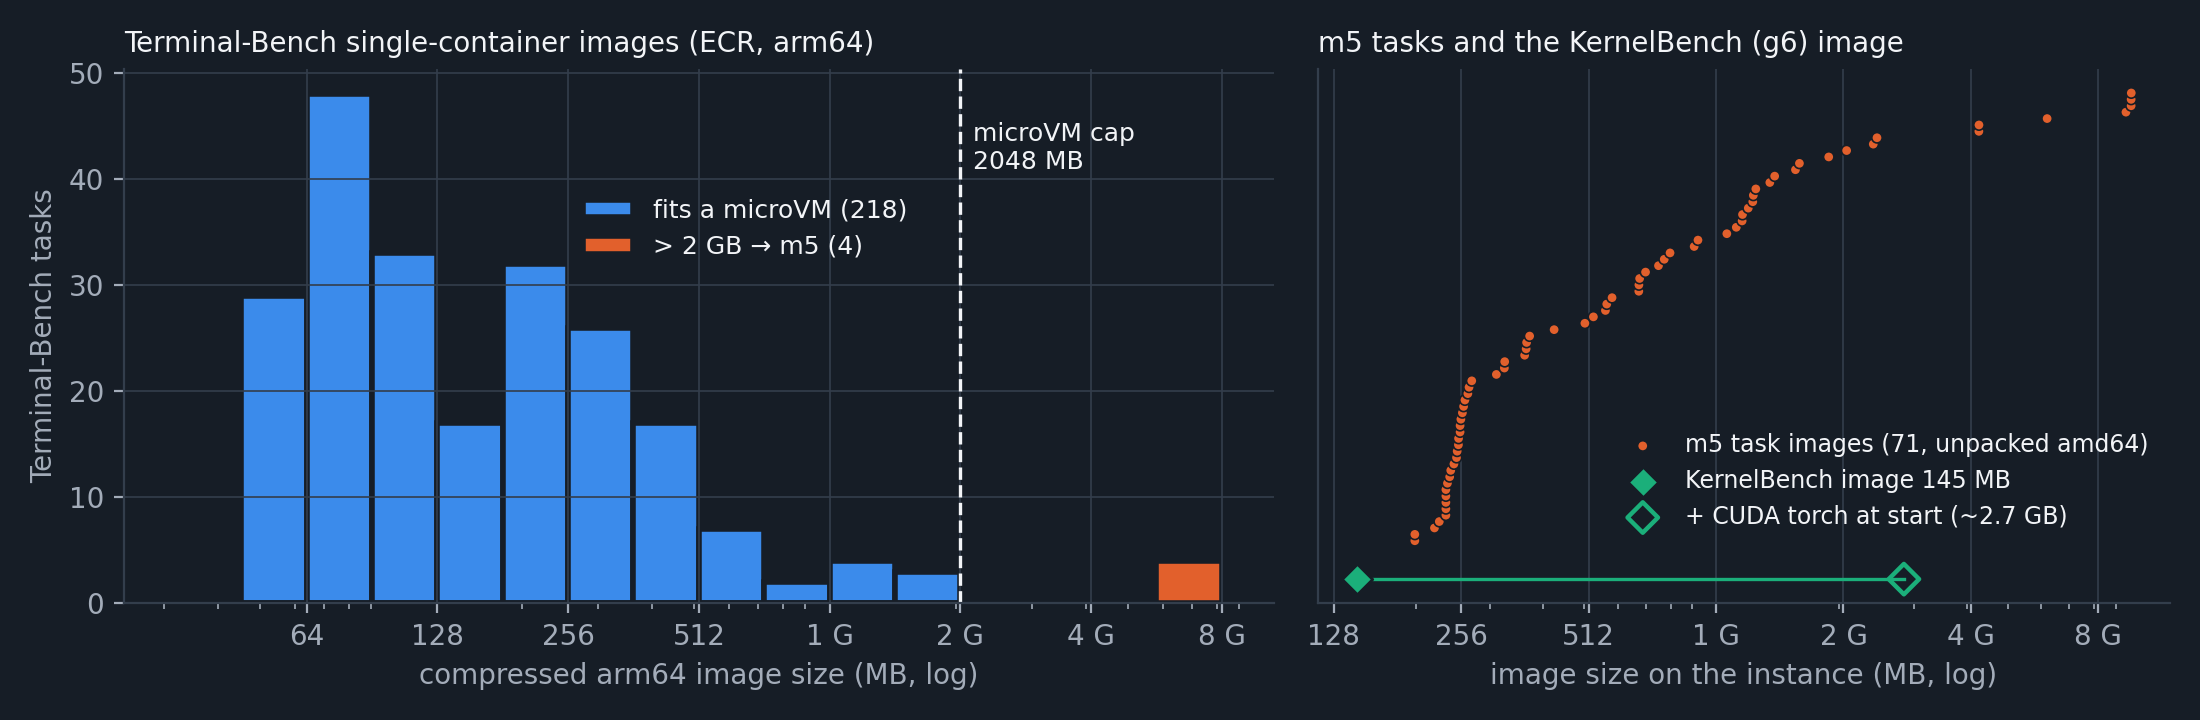
\includegraphics[width=0.88\textwidth]{fig_image_sizes.png}\par
\raggedright\vspace{1mm}
\begin{columns}[T]
\column{0.48\textwidth}
\begin{itemize}\scriptsize\setlength{\itemsep}{0.5mm}
\item \textbf{arm64 microVM images:} p50 \textbf{127\,MB}, p95 620\,MB, largest that fits 2.0\,GB.
\item \textbf{4 tasks are 6.5--6.7\,GB} (\tb{mteb-*}, \tb{png-generation}): no microVM can take them.
\end{itemize}
\column{0.48\textwidth}
\begin{itemize}\scriptsize\setlength{\itemsep}{0.5mm}
\item \textbf{m5 images} (unpacked, amd64): p50 525\,MB, up to 9.8\,GB; the m5 has a 40\,GB disk.
\item \textbf{KernelBench:} the 2\,GB cap also applies to capacity-provider Runtimes, so the image is
  145\,MB and installs CUDA torch ($\sim$2.7\,GB) at container start ($\sim$90\,s).
\end{itemize}
\end{columns}
\src{\tb{images.csv} (ECR compressed size), \tb{images\_docker.csv} (\tb{docker image inspect}); \tb{make\_figures.py}; checked 4 Oct 2026.}
\end{frame}

%====================================================================
\begin{frame}{Together they hit 16 challenges every agentic-RL sandbox has to solve}
\flabel{fr:chal}
\tabcap{The challenges, which benchmark exposes each, and what it looked like here}
\tiny\setlength{\tabcolsep}{3pt}
\begin{tabularx}{\textwidth}{@{}P{0.02\textwidth} P{0.24\textwidth} P{0.07\textwidth} Y@{}}
\toprule
& \textbf{Challenge} & \textbf{Exposed by} & \textbf{What it looked like in this demo}\\
\midrule
\grp{4}{Environments: every task needs its own machine}\\
1 & \textbf{One environment per task} & TB & 241 tasks, 241 Dockerfiles: no shared image can serve them\\
2 & \textbf{Image size limits} & TB, KB & microVM cap 2\,GB; 4 tasks are 6.5--6.7\,GB; CUDA torch alone is $\sim$2.7\,GB\\
3 & \textbf{CPU architecture} & TB & microVMs are arm64 only; 4 tasks need x86 (QEMU, x86 assembly)\\
4 & \textbf{Multi-container tasks} & TB & 12 tasks need sidecars (Postgres, web servers) on a private network\\
5 & \textbf{Missing privileges} & TB & microVMs drop all Linux capabilities: 21 reference solutions fail there\\
6 & \textbf{Accelerators} & KB & GPUs only on capacity-provider Instances, one session per instance; g6 capacity ran out for hours\\
\grp{4}{Speed at RL scale: the trainer must never wait for a sandbox}\\
7 & \textbf{Cold starts on the critical path} & all & opens take 2\,s (microVM), $\sim$35--68\,s (m5), $\sim$2.5\,min (g6) vs a $\sim$20\,s episode\\
8 & \textbf{Idle reclaim} & TB & an idle microVM session is wiped after 15\,min; pre-opened ones idled up to 16.5\,min\\
9 & \textbf{Concurrency and quotas} & TB, KB & 32 episodes per step plus look-ahead; Runtime, vCPU and session quotas; no fallback between GPU types\\
10 & \textbf{Long or hung tool calls} & TB & 4-min commands, detached children, non-idempotent retries stalled an eval\\
\grp{4}{Correct rewards: the score must mean what it says}\\
11 & \textbf{Isolation between episodes} & TB & the agent rewrites the OS; any reuse risks leaking state into the next score\\
12 & \textbf{Reward integrity} & TB, KB & tests must stay hidden; copying \tb{Model} onto CUDA ``passed'' KernelBench\\
13 & \textbf{Untrustworthy tasks} & TB & deleted repos, 404 downloads, oracles that fail on a substrate: 241 $\rightarrow$ 193 usable\\
14 & \textbf{Sparse reward, no gradient} & TB, KB & all-or-nothing scores: no GRPO gradient in 32 of 48 steps\\
\grp{4}{Operating it: safe, visible, and cheap}\\
15 & \textbf{Network and security} & all & the agent loop runs in the sandbox and must reach the trainer, with no public ports\\
16 & \textbf{Clean-up, cost and visibility} & all & leftover instances after a crash; g6 instances do not show in your EC2 console\\
\bottomrule
\end{tabularx}
\par\vspace{1mm}
{\scriptsize\textbf{Why both benchmarks:} Terminal-Bench brings the \textbf{variety of environments} (1--5, 8, 10--11, 13), KernelBench the
\textbf{hardware} (2, 6) and a \textbf{measured, gameable reward} (12, 14). Neither alone exposes all 16; together they need all three substrates.\par}
\src{Sections 2--4 of this deck; \sref{fr:lessons} (Lessons); \tb{images.csv}, \tb{oracle.csv}; checked 6 Oct 2026.}
\end{frame}

%====================================================================
\sect{The hybrid solution}

\begin{frame}{How the demo answers each challenge, at a glance}
\flabel{fr:sol}
\begin{columns}[T]
\column{0.49\textwidth}
\textbf{\footnotesize Environments}
\begin{itemize}\tiny\setlength{\itemsep}{0.3mm}
\item[1] \textbf{One image + one Runtime per task}, built from the task's own Dockerfile plus one small wrapper (\sref{fr:route}).
\item[2] \textbf{Route by measured size}: $>$ 2\,GB goes to an m5; the GPU image stays small and installs CUDA torch at start.
\item[3] \textbf{Route by build result}: arm64 failures run on x86 m5s.
\item[4] \textbf{Whole compose project on its own m5}, rewritten per episode so names, ports and mounts never collide.
\item[5] \textbf{Validate every oracle} on its substrate; microVM failures are retried on an m5 and kept where they pass.
\item[6] \textbf{g6 capacity provider}, one fresh Instance per episode; list the GPU type that has capacity first.
\end{itemize}
\textbf{\footnotesize Speed at RL scale}
\begin{itemize}\tiny\setlength{\itemsep}{0.3mm}
\item[7] \textbf{Look-ahead pre-open}: boot the next 2 batches (5 for m5 and g6) while the current one runs (\sref{fr:preopen}).
\item[8] \textbf{Heartbeat}: ping idle pre-opened sessions at half the idle timeout.
\item[9] \textbf{Per-substrate caps} (m5 instances, g6 sessions), sized to the look-ahead; quotas checked up front (\sref{fr:quotas}).
\item[10] \textbf{Per-command timeouts}, no retry of non-idempotent \tb{exec}, the harness never waits on detached children.
\end{itemize}
\column{0.49\textwidth}
\textbf{\footnotesize Correct rewards}
\begin{itemize}\tiny\setlength{\itemsep}{0.3mm}
\item[11] \textbf{Fresh sandbox per episode}; a warm m5 is reused only after a \textbf{verified} reset (\sref{fr:sessions}).
\item[12] \textbf{Tests injected only after the agent stops}; random-named checker with a nonce'd PASSED line; KernelBench needs a \textbf{1.10$\times$ speedup} for full reward.
\item[13] \textbf{Routing is data}: only tasks whose oracle passes are trained on; broken upstream tasks are dropped.
\item[14] \textbf{Denser reward}: partial credit for passed tests in training (eval stays 0/1), the 0 / 0.5 / 1 KernelBench gate, and dropping tasks whose reward never varies (\sref{fr:reward}).
\end{itemize}
\textbf{\footnotesize Operating it}
\begin{itemize}\tiny\setlength{\itemsep}{0.3mm}
\item[15] \textbf{Private by design}: VPC Runtimes, SG-to-SG rules, m5 agent behind a shared secret, no public ports (\sref{fr:sec}).
\item[16] \textbf{Close on every path}: stop sessions at episode end, terminate m5s at exit, a dead-man switch on each m5, \tb{6\_cleanup.sh}; CloudTrail timeline for the g6s.
\end{itemize}
\vspace{1mm}
\colorbox{panel}{\parbox{\dimexpr\linewidth-2\fboxsep}{\scriptsize\textbf{One RL code path:} none of the 16 answers touches slime, the agent loop or the grader; they all live in the sandbox tier.}}
\end{columns}
\src{Demo README; \tb{terminalbench\_pool.py}, \tb{ec2\_episode\_sandbox.py}, \tb{deploy\_gpu\_tasks.py}, \tb{filter\_by\_history.py}; checked 6 Oct 2026.}
\end{frame}

%====================================================================
\begin{frame}{The demo: use case covered, why this demo, design considerations}
\flabel{fr:hybrid}
\scriptsize\setlength{\tabcolsep}{4pt}
\tabcap{The demo in three answers}
\begin{tabularx}{\textwidth}{@{}P{0.17\textwidth}Y@{}}
\toprule
\textbf{Use case covered} & Agentic RL on benchmarks whose environments \textbf{do not all fit one sandbox product}:
small single containers, multi-container compose projects, x86-only or multi-GB images, root-level tasks, and GPU kernels.\\
\textbf{Why this demo} & It trains on \hl{the whole usable corpus} (193 Terminal-Bench + 50 KernelBench) instead of the 165
tasks microVMs alone can validate, and shows the sandbox tier can be \textbf{heterogeneous without touching the RL side}.
\tb{eval/terminalbench} stays the same held-out microVM set as the earlier microVM-only demo.\\
\textbf{Design considerations} &
\textbf{One protocol, three transports}: every image is the task's Dockerfile + the same wrapper (\tb{/opt/acs/py} + stdlib
\tb{acs\_http\_server.py}); AgentCore invokes it on a microVM or g6, the trainer POSTs to it on an m5
\textperiodcentered{} \textbf{routing is data} (\sref{fr:route})
\textperiodcentered{} \textbf{one session per sandbox} (\sref{fr:sessions})
\textperiodcentered{} \textbf{per-episode compose rewrite}: fixed names, host ports and \tb{./} mounts made unique; privileged, host network, \tb{docker.sock} refused
\textperiodcentered{} \textbf{hidden tests stay hidden}: task dirs reach the m5 without \tb{tests/} or the solution
\textperiodcentered{} \textbf{microVM images reused} byte-for-byte from the shared \tb{acs-tb-*} ECR repos.\\
\textbf{Rejected} & Compose on AgentCore (no capabilities, no daemon) \textperiodcentered{} flattening sidecars into one session
(changes the task) \textperiodcentered{} the g6e trainer as Docker host (it trains) \textperiodcentered{} ECS/EKS (more moving parts than
EC2 for 30 tasks) \textperiodcentered{} g5 for KernelBench (works, but g6 is cheaper: \$0.80 vs \$1.01/h).\\
\bottomrule
\end{tabularx}
\src{\tb{code/demos/demo\_terminalbench\_kernelbench/README.md}; \tb{docs/terminalbench-kernelbench-demo-plan.md}, \tb{docs/docker-compose-on-aws.md}; checked 4 Oct 2026.}
\end{frame}

%====================================================================
\begin{frame}{One trainer, one router, three sandbox substrates}
\flabel{fr:arch}
\figcap{Components: the trainer routes each row; the agent loop runs inside the sandbox and dials back}
\centering
\begin{tikzpicture}[node distance=4mm]
\node[box,minimum width=44mm,minimum height=30mm,align=left] (tr) {%
  \textbf{\small g6e.48xlarge trainer} (8$\times$L40S)\\[1mm]
  slime fully-async GRPO, Qwen3-4B\\
  4 GPUs train $\cdot$ 4 GPUs SGLang\\
  \tb{AnthropicAdapter} per engine\\[1mm]
  \textbf{\tb{TerminalBenchPool}}\\
  route map $\cdot$ pre-open $\cdot$ gates\\
  grader (hidden tests)};
\node[box,draw=cat2,right=26mm of tr,yshift=13mm,text width=54mm,align=left] (mv) {%
  \textbf{\textcolor{cat2}{AgentCore microVM}}\quad 218 Runtimes \tb{acs\_tbh\_*}\\
  arm64, $\le$ 2\,GB $\cdot$ 1 session = 1 microVM};
\node[box,draw=cat1,right=26mm of tr,text width=54mm,align=left] (m5) {%
  \textbf{\textcolor{cat1}{m5 EC2}}\quad warm pool, $\le$ 24 \tb{m5.xlarge}\\
  Docker + compose agent $\cdot$ 1 session = 1 VM};
\node[box,draw=cat3,right=26mm of tr,yshift=-13mm,text width=54mm,align=left] (g6) {%
  \textbf{\textcolor{cat3}{AgentCore g6 Instance}}\quad \tb{acs\_tbhgpu\_kernelbench}\\
  g6.xlarge L4 $\cdot$ 1 session = 1 instance};
\draw[arr,cat2] (tr.east)+(0,4mm) -- node[above,sloped,font=\tiny,text=inkmuted]{InvokeAgentRuntime} (mv.west);
\draw[arr,cat1] (tr.east) -- node[above,font=\tiny,text=inkmuted]{EC2 API + HTTP} (m5.west);
\draw[arr,cat3] (tr.east)+(0,-4mm) -- node[below,sloped,font=\tiny,text=inkmuted]{InvokeAgentRuntime} (g6.west);
\node[font=\tiny,text=inkmuted,align=left,right=2mm of m5] {agent loop runs\\here and calls\\\tb{/v1/messages}\\back over the VPC};
\end{tikzpicture}
\par\vspace{2mm}\raggedright
\begin{columns}[T]
\column{0.32\textwidth}
\scriptsize\textbf{\textcolor{cat2}{microVM}:} 163 tasks. Managed by AgentCore; an idle session is wiped after 15\,min, so a heartbeat keeps pre-opened ones alive.
\column{0.32\textwidth}
\scriptsize\textbf{\textcolor{cat1}{m5}:} 30 tasks. \textbf{Our code} launches and terminates them (boto3, the g6e's role), from a baked AMI; images from ECR.
\column{0.32\textwidth}
\scriptsize\textbf{\textcolor{cat3}{g6}:} KernelBench. In an AgentCore-managed account: \textbf{not in our EC2 console}; one CloudWatch log stream per session.
\end{columns}
\src{\tb{agentcore\_slime\_demo/\{terminalbench\_pool, docker\_compose\_sandbox, ec2\_episode\_sandbox\}.py}, \tb{image\_routing.py}, \tb{run.sh}; checked 4 Oct 2026.}
\end{frame}

%====================================================================
\begin{frame}{Which substrate does a task get? Four questions, answered from data}
\flabel{fr:route}
\figcap{The routing decision, with the number of Terminal-Bench tasks on each branch}
\centering
\begin{tikzpicture}[x=29mm,y=13mm, every node/.style={font=\scriptsize}]
\tikzset{q/.style={box,text width=22mm,minimum height=10mm}, o/.style={box,text width=22mm,minimum height=9mm}}
\node[q] (q1) at (0,0) {Needs a GPU?};
\node[q] (q2) at (1,0) {One container only?};
\node[q] (q3) at (2,0) {Builds for arm64 and $\le$ 2\,GB?};
\node[q] (q4) at (3,0) {Reference solution passes on a microVM?};
\node[o,draw=cat2] (mv) at (4,0) {\textcolor{cat2}{\textbf{microVM}}\\163 usable};
\node[o,draw=cat3] (g6) at (0,-1.3) {\textcolor{cat3}{\textbf{g6}}\\KernelBench (50)};
\node[o,draw=cat1] (c) at (1,-1.3) {\textcolor{cat1}{\textbf{m5}}: compose (12)};
\node[o,draw=cat1] (b) at (2,-1.3) {\textcolor{cat1}{\textbf{m5}}: x86 or big (11)};
\node[o,draw=cat1] (rt) at (3,-1.3) {\textcolor{cat1}{\textbf{m5}} retry (53)};
\node[box,draw=cat1,text width=62mm] (m5) at (2,-2.45) {every m5 candidate is built on the m5 builder (71 of 78 build) and must pass its oracle there: \textcolor{cat1}{\textbf{30 usable}}};
\draw[arr] (q1) -- node[above]{no} (q2); \draw[arr] (q2) -- node[above]{yes} (q3);
\draw[arr] (q3) -- node[above]{yes} (q4); \draw[arr] (q4) -- node[above]{yes} (mv);
\draw[arr] (q1) -- node[right]{yes} (g6); \draw[arr] (q2) -- node[right]{no} (c);
\draw[arr] (q3) -- node[right]{no} (b); \draw[arr] (q4) -- node[right]{no} (rt);
\draw[arr] (c) -- (m5); \draw[arr] (b) -- (m5); \draw[arr] (rt) -- (m5);
\end{tikzpicture}
\par\vspace{1mm}\raggedright
\begin{itemize}\scriptsize\setlength{\itemsep}{0.4mm}
\item \textbf{193 of 241 Terminal-Bench tasks are usable} (163 + 30) vs 165 with microVMs alone. Every answer is measured: \tb{manifest.json} (containers), \tb{images.csv} (build, size), \tb{oracle.csv} (oracle). \tb{image\_routing.py} refuses a task with no route.
\item \textbf{Not usable (48):} 5 build nowhere (e.g.\ \tb{fix-git}: its GitHub repo was deleted); the rest fail their oracle on every substrate, incl.\ the 4 big \tb{mteb-*}/\tb{png-generation} images.
\end{itemize}
\src{\tb{terminalbench/tasks/\{manifest.json, images.csv, images\_docker.csv, oracle.csv, route\_by\_image.json\}}; checked 5 Oct 2026.}
\end{frame}

%====================================================================
\begin{frame}{One episode is the same five steps on every substrate}
\flabel{fr:pipeline}
\tabcap{What \tb{TerminalBenchPool} does per episode, by substrate}
\scriptsize\setlength{\tabcolsep}{3pt}
\begin{tabularx}{\textwidth}{@{}P{0.13\textwidth}YYY@{}}
\toprule
\textbf{Step} & \textbf{\textcolor{cat2}{microVM}} & \textbf{\textcolor{cat1}{m5 EC2 (warm)}} & \textbf{\textcolor{cat3}{g6 Instance}}\\
\midrule
1. Route & \tb{arn:\ldots/acs\_tbh\_<task>} & \tb{docker://<ip>:18300/<task>} & \tb{gpu:arn:\ldots/}\newline\tb{acs\_tbhgpu\_kernelbench}\\
2. Open (ahead) & new \tb{runtimeSessionId}; first invoke boots the microVM & idle VM (prefer one holding the images) or \tb{run\_instances}; ECR pull; \tb{compose up} & new session id; first invoke launches a g6, then torch install\\
3. Agent loop & \multicolumn{3}{>{\centering\arraybackslash}X}{mini\_claude (\tb{bash} / \tb{write\_file} / \tb{read\_file}), up to 8 turns $\times$ 1024 tokens, \textbf{inside the sandbox}, calling the trainer's adapter}\\
4. Grade & inject \tb{tests/}, run pytest & same, in the client & hidden checker: correctness + \tb{speedup=}\\
5. Close & \tb{StopRuntimeSession} & \tb{compose down -v} + \tb{reset\_check}; clean $\rightarrow$ pool, dirty $\rightarrow$ terminate & \tb{StopRuntimeSession} (instance released)\\
\midrule
Open cost (smoke 6, p50) & \textbf{2\,s} & \textbf{68\,s} (launch or reuse, pull, \tb{compose up}) & \textbf{135\,s} (boot + $\sim$90\,s torch)\\
Episode p50 & 24\,s (agent 12\,s, grade 9\,s) & 69\,s (agent 14\,s, grade 7\,s) & 30\,s (first command $\rightarrow$ stop; p90 41\,s)\\
\bottomrule
\end{tabularx}
\par\vspace{1mm}
\plainen{the RL code never asks which substrate it is on; only the open cost differs (2\,s to over 2\,min).}
\src{\tb{logs/smoke6-hybrid\_*.log} (\tb{[demo]} \tb{agent\_ms}, \tb{grade\_ms}, \tb{episode\_ms}, \tb{open\_ms}); m5 per-episode probe; checked 4 Oct 2026.}
\end{frame}

%====================================================================
\begin{frame}{Sessions and instances: one session per instance, three lifecycles}
\flabel{fr:sessions}
\begin{columns}[T]
\column{0.54\textwidth}
\tabcap{Who owns each instance, and how it ends}
\scriptsize\setlength{\tabcolsep}{3pt}
\begin{tabularx}{\linewidth}{@{}P{0.20\linewidth}YYY@{}}
\toprule
& \textbf{\textcolor{cat2}{microVM}} & \textbf{\textcolor{cat1}{m5}} & \textbf{\textcolor{cat3}{g6}}\\
\midrule
Managed by & AgentCore & \textbf{our trainer} & AgentCore\\
Reused? & no, fresh & yes, after a verified reset & no, fresh\\
Isolation & own kernel & own VM per session & own instance\\
Visible in & CloudWatch & our EC2 console & CloudWatch only\\
Ends by & stop / 15-min idle & 5 ways (right) & stop / 600\,s idle\\
Peak live (\tb{train48}) & 88 & 24 & 36\\
\bottomrule
\end{tabularx}
\par\vspace{2mm}
\tabcap{Warm m5 pool in smoke 6}
\scriptsize
\begin{tabular}{@{}l r@{}}
\toprule
instances launched / episodes on a reused one & 24 / 10\\
pool peak (cap \tb{TB\_M5\_MAX\_INSTANCES}) & 24 (24)\\
dirty resets / retired & \hl{0 / 0}\\
\bottomrule
\end{tabular}
\column{0.42\textwidth}
\begin{itemize}\scriptsize\setlength{\itemsep}{0.8mm}
\item \textbf{Verified reset} after every m5 episode: no containers, volumes or extra networks, empty episode
  dir, $\ge$ 8\,GB disk. Dirty or unhealthy $\rightarrow$ terminated, never reused. No periodic recycle.
\item \textbf{m5 termination, 5 ways:} trainer \tb{atexit}; \tb{5\_run.sh} \tb{gc-episodes}; next pool start;
  \tb{6\_cleanup.sh}; a \textbf{dead-man switch} (no trainer call for 30\,min $\rightarrow$ the VM shuts
  itself down = terminate).
\item \textbf{g6:} a launch per session, so a pre-open must start $\sim$2.5\,min early (\sref{fr:preopen}).
\item Isolation and hardening details: \sref{fr:harden}.
\end{itemize}
\end{columns}
\src{\tb{agentcore\_slime\_demo/ec2\_episode\_sandbox.py} (\tb{WarmPool}); \tb{logs/smoke6-hybrid\_*}, \tb{logs/train48-hybrid\_*} (\tb{[sbx-op]}, \tb{warm\_reused}); checked 4 Oct 2026.}
\end{frame}

%====================================================================
\begin{frame}{Pre-open hides cold starts from 2\,s to 2.5\,min behind the running batch}
\flabel{fr:preopen}
\figcap{Median wait for the sandbox at episode start: measured with pre-open vs the open time it hides}
\centering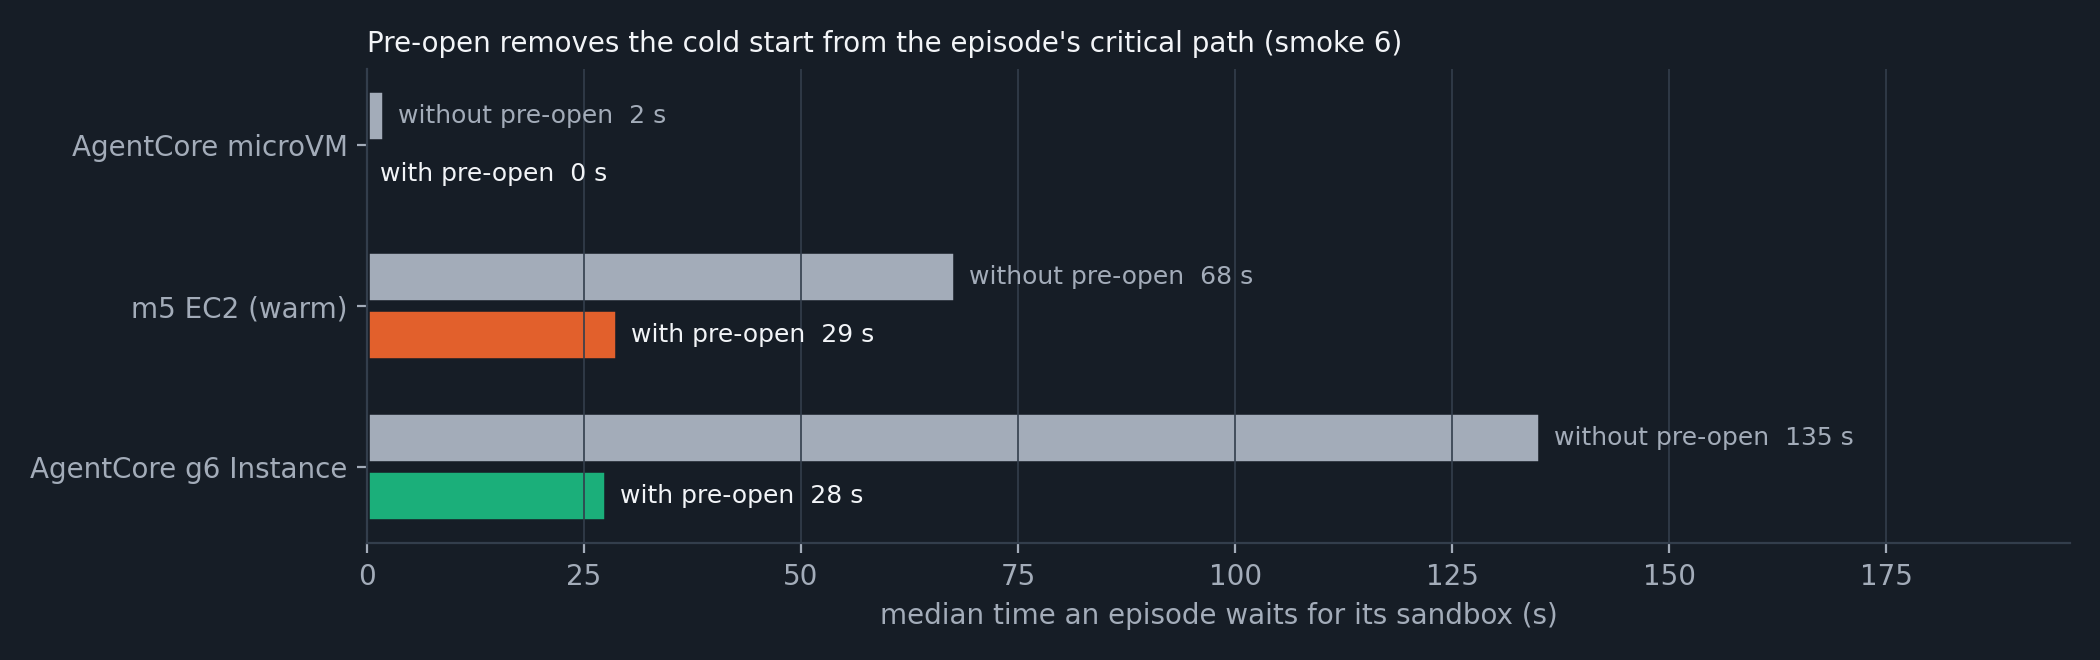
\includegraphics[width=0.84\textwidth]{fig_preopen.png}\par
\raggedright\vspace{1mm}
\begin{columns}[T]
\column{0.50\textwidth}
\tabcap{Smoke 6, by substrate}
\tiny\setlength{\tabcolsep}{3pt}
\begin{tabularx}{\linewidth}{@{}Y r r r r@{}}
\toprule
& \textbf{n} & \textbf{no wait} & \textbf{wait p90} & \textbf{saved}\\
\midrule
\textcolor{cat2}{microVM} (2 batches ahead) & 177 & 121 & 5.6\,s & 4\,min\\
\textcolor{cat1}{m5} (5 batches ahead) & 34 & 16 & 61\,s & 23\,min\\
\textcolor{cat3}{g6} (5 batches ahead) & 52 & 22 & 100\,s & \hl{80\,min}\\
\bottomrule
\end{tabularx}
\column{0.46\textwidth}
\tabcap{g6 session cap vs start wait}
\tiny\setlength{\tabcolsep}{3pt}
\begin{tabular}{@{}l r r r@{}}
\toprule
\textbf{Run} & \textbf{cap} & \textbf{wait p50} & \textbf{no wait}\\
\midrule
smoke 4 & 8 & 240\,s & 0 / 76\\
smoke 5 & 16 & 82\,s & 5 / 36\\
smoke 6 & 32 & \hl{28\,s} & 22 / 52\\
\bottomrule
\end{tabular}
\par\vspace{0.5mm}{\tiny A cap of 8 equals one group, so nothing could open ahead.}
\end{columns}
\src{\tb{logs/smoke\{4mix,5,6\}-hybrid\_*.log} (\tb{[demo]} \tb{open\_wait\_ms}, \tb{open\_ms}); ``saved'' = $\sum$ max(0, open $-$ wait); \tb{make\_figures.py}; checked 4 Oct 2026.}
\end{frame}

%====================================================================
\begin{frame}{Instances during training: 2,020 microVMs, 129 m5 and 546 g6 in one run}
\flabel{fr:instances}
\figcap{Sandboxes alive at once over the 48-step run (train48 run 2), sampled every 10\,s}
\centering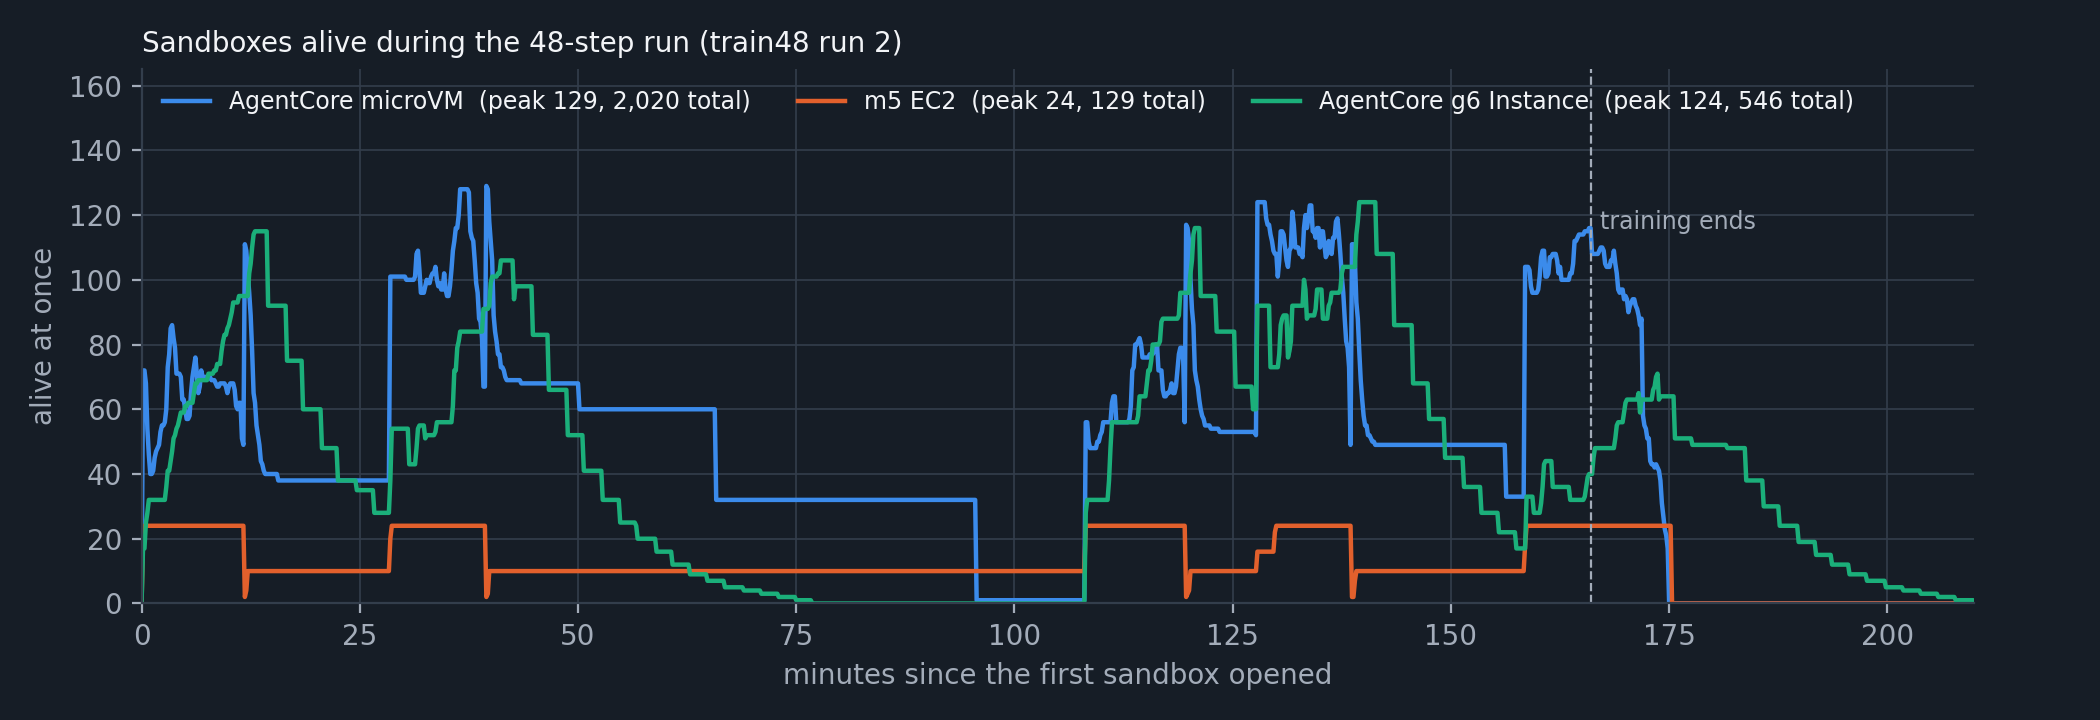
\includegraphics[width=0.78\textwidth]{fig_instances.png}\par
\raggedright\vspace{1mm}
\begin{columns}[T]
\column{0.50\textwidth}
\tabcap{Per substrate, whole run}
\tiny\setlength{\tabcolsep}{3pt}
\begin{tabularx}{\linewidth}{@{}Y r r r@{}}
\toprule
& \textbf{total} & \textbf{peak} & \textbf{mean}\\
\midrule
\textcolor{cat2}{microVM} (one per session) & 2,020 & 129 & 57\\
\textcolor{cat1}{m5} (warm pool, 407 sessions) & 129 & 24 & 14\\
\textcolor{cat3}{g6} (one per session) & 546 & 124 & 46\\
\bottomrule
\end{tabularx}
\column{0.46\textwidth}
\tabcap{Why g6 peaks above its session cap of 32}
\tiny
A g6 session lasts \textbf{3\,min} (median), but AgentCore keeps its Instance for \hl{15\,min}: it is
reclaimed about 12\,min after the session stops. Most g6 time is idle, and the last Instances
outlive training by 44\,min. m5 is reused after a verified reset, so 129 hosts served 407 sessions.
\end{columns}
\src{\tb{logs/train48-hybrid\_*.\{sessions,sandbox\_ops,instances\}.csv}; m5/g6 lifetimes from CloudTrail (\tb{instance\_timeline.py}); \tb{make\_figures.py}; checked 5 Oct 2026.}
\end{frame}

%====================================================================
\begin{frame}{Security and network: private by design, no public ports}
\flabel{fr:sec}
\tabcap{Where each component runs and who can reach it}
\scriptsize\setlength{\tabcolsep}{3pt}
\begin{tabularx}{\textwidth}{@{}P{0.16\textwidth}P{0.27\textwidth}YP{0.20\textwidth}@{}}
\toprule
\textbf{Component} & \textbf{Placement} & \textbf{Inbound allowed} & \textbf{Outbound}\\
\midrule
\textcolor{cat2}{microVM} / \textcolor{cat3}{g6} sessions & AgentCore \textbf{VPC mode}, our private \tb{acs-egress-<az>} subnets & none: reached only through the IAM-signed AgentCore API & existing NAT (pip at grading); AWS via private endpoints\\
\textcolor{cat1}{m5} episodes + builder & private egress subnet, \textbf{no public IP} & tcp 18300 (agent) and 32768--60999 (episode client) \textbf{from the trainer's SG only}; no SSH rule & existing NAT; IMDS blocked from containers\\
Trainer (g6e) & our VPC & tcp 18100--18163 (model adapters) \textbf{from the Runtime and m5 SGs only} & --\\
\bottomrule
\end{tabularx}
\par\vspace{2mm}
\begin{columns}[T]
\column{0.48\textwidth}
\begin{itemize}\scriptsize\setlength{\itemsep}{0.7mm}
\item \textbf{Private endpoints} (created by step 4): \tb{ecr.api}, \tb{ecr.dkr}, \tb{logs}, \tb{sts}, \tb{bedrock-agentcore}, and an S3 gateway for ECR layers.
\item \textbf{No NAT gateway is created}; an existing one is required for tasks whose tests install packages. \tb{RUNTIME\_EGRESS=none} = no internet at all.
\item \textbf{No credentials worth stealing} in a sandbox: the m5 role can only pull its own images (\sref{fr:iam}).
\end{itemize}
\column{0.48\textwidth}
\begin{itemize}\scriptsize\setlength{\itemsep}{0.7mm}
\item \textbf{The m5 agent API} needs a per-instance secret; it is plain HTTP inside the VPC, limited by the SG-to-SG rule.
\item \textbf{Ray dashboard} (8265) listens on the trainer but no SG rule exposes it.
\item \textbf{Dev-account note:} our trainer host has a public IP and \textbf{SSH open to 0.0.0.0/0}. The solution does not need it: restrict it to your IP or use SSM Session Manager.
\end{itemize}
\end{columns}
\src{\tb{deploy/agentcore\_deploy.py} (\tb{RUNTIME\_NETWORK=VPC}, \tb{vpc\_network}, endpoints), \tb{deploy/m5\_host.py} (SG rules, \tb{AssociatePublicIpAddress=False}); \tb{aws ec2 describe-security-groups}; checked 5 Oct 2026.}
\end{frame}

%====================================================================
\sect{Results}

\begin{frame}{Reliability: 12 infra errors in 5,332 episodes, on all three substrates}
\flabel{fr:rel}
\tabcap{Smoke runs (4 Oct) and the 48-step runs (4--5 Oct 2026): episodes (train + eval) / infra errors}
\scriptsize\setlength{\tabcolsep}{4pt}
\begin{tabularx}{\textwidth}{@{}P{0.11\textwidth}P{0.12\textwidth}P{0.10\textwidth}P{0.10\textwidth}Y@{}}
\toprule
\textbf{Run} & \textbf{\textcolor{cat2}{microVM}} & \textbf{\textcolor{cat1}{m5}} & \textbf{\textcolor{cat3}{g6}} & \textbf{Run result and what changed after it}\\
\midrule
smoke 2 & 401 / 1 & 88 / 0 & -- & final checkpoint save hung (\tb{pidfd\_getfd} EPERM) $\rightarrow$ allocator setting made opt-in\\
smoke 3 & 382 / \hl{0} & 88 / \hl{0} & -- & \textbf{passed}, 53\,GB checkpoint; m5 per-episode $\rightarrow$ warm pool next\\
smoke 4 & 322 / 1 & 58 / 1 & 75 / 0 & \textbf{passed}; KernelBench added; g6 cap 8 too small\\
smoke 5 & 157 / 0 & 34 / 0 & 36 / 0 & \textbf{passed}; speedup-gated reward, g6 cap 16\\
smoke 6 & 177 / 1 & 34 / 0 & 52 / 0 & \textbf{passed}; g6 cap 32, 5 batches ahead\\
train48 run 1 & 700 / 1 & 76 / 0 & 160 / 0 & 20 steps, then the eval deadlock $\rightarrow$ warm pool tracks the holding loop\\
train48 run 2 & 1{,}795 / 5 & 293 / 2 & 404 / 0 & \textbf{passed}, 48 of 48 steps; all 7 errors are grading failures (HTTP 500)\\
\midrule
\textbf{total} & 3{,}934 / 9 & 671 / 3 & 727 / 0 & \hl{5{,}332 episodes, 12 infra errors (0.2\,\%)}\\
\bottomrule
\end{tabularx}
\par\vspace{2mm}
\begin{columns}[T]
\column{0.48\textwidth}
\begin{itemize}\scriptsize\setlength{\itemsep}{0.8mm}
\item \textbf{Every run since smoke 3 finished} except \tb{train48} run 1 (\tb{Job \ldots{} succeeded}); smokes 3--4 saved a 53\,GB checkpoint.
\item \textbf{11 of 12 errors are grading failures} (\tb{grade\_exit=-1}: the sandbox returned HTTP 500 to the test run), 7 of them on two tasks: \tb{solve-maze-challenge} (4), \tb{build-initramfs-qemu} (3).
\item \textbf{0 dirty warm-m5 resets}; all m5s terminated at exit.
\end{itemize}
\column{0.48\textwidth}
\begin{itemize}\scriptsize\setlength{\itemsep}{0.8mm}
\item \textbf{Not counted:} 25 episodes still in flight when run 2 exited (pre-opened for batches that never ran). A bug: the look-ahead ran on past the last step. Fixed: it is now stopped after the last rollout, its sessions closed (\tb{last\_rollout.py}).
\item Bugs found on the way and their fixes: \sref{fr:lessons}.
\end{itemize}
\end{columns}
\src{\tb{logs/\{smoke\{2,3,4mix,5,6\},train48\}-hybrid\_*.log} (\tb{[demo] episode\_end} \tb{infra\_error=}, \tb{cancelled=}); \tb{make\_figures.py} $\rightarrow$ \tb{data.json} (runs); checked 5 Oct 2026.}
\end{frame}

%====================================================================
\begin{frame}{Reward design: KernelBench needed a speedup gate to give a gradient}
\flabel{fr:reward}
\begin{columns}[T]
\column{0.52\textwidth}
\tabcap{Reward per run (TB: solved / episodes; KB: count per reward)}
\scriptsize\setlength{\tabcolsep}{3pt}
\begin{tabularx}{\linewidth}{@{}P{0.16\linewidth}YYY@{}}
\toprule
\textbf{Run} & \textbf{\textcolor{cat2}{TB microVM}} & \textbf{\textcolor{cat1}{TB m5}} & \textbf{\textcolor{cat3}{KernelBench}}\\
\midrule
smoke 3 & 16 / 382 & 0 / 88 & --\\
smoke 4 & 13 / 322 & 0 / 58 & 1: 48, 0: 27\\
smoke 5 & 6 / 157 & 0 / 34 & 0.5: 26, 0: 10\\
smoke 6 & 4 / 177 & 0 / 34 & 1: 8, 0.5: 34, 0: 10\\
\midrule
eval (s6) & 1 / 62 & 0 / 10 & mean 0.45\\
\bottomrule
\end{tabularx}
\column{0.44\textwidth}
\begin{itemize}\scriptsize\setlength{\itemsep}{1mm}
\item \textbf{GRPO learns only from groups with mixed rewards.} All-0 or all-1 groups give no gradient.
\item \textbf{KernelBench, correctness only} (smoke 4): copying \tb{Model} onto CUDA passed, so 64\,\% scored 1.
\item \textbf{Speedup gate} (smoke 5--6): 1 only if $\ge$ 1.10$\times$ faster. Copies measure 1.00--1.03$\times$,
  so the bar is above noise. Smoke 6 had all three reward levels; best kernel 1.38$\times$.
\item \textbf{Terminal-Bench is all-or-nothing}: a 4B model solves 2--4\,\% on microVMs and \textbf{0\,\%} of the
  harder m5 tail, so most groups carry no gradient.
\end{itemize}
\end{columns}
\src{\tb{logs/smoke\{3,4mix,5,6\}-hybrid\_*.\{log,eval.csv\}} (\tb{solved=}, \tb{reward=}, \tb{speedup=}); checked 4 Oct 2026.}
\end{frame}

%====================================================================
\begin{frame}{Learning: 48 steps ran clean, but most steps carried no gradient}
\flabel{fr:train}
\begin{columns}[T]
\column{0.52\textwidth}
\tabcap{The two 48-step runs (\tb{RB=4}, \tb{NS=8}: 32 episodes per step)}
\scriptsize\setlength{\tabcolsep}{3pt}
\begin{tabularx}{\linewidth}{@{}Y r r@{}}
\toprule
& \textbf{run 1} & \textbf{run 2}\\
\midrule
started (UTC) & 4 Oct 15:24 & 5 Oct 00:56\\
steps done & 20 of 48 & \hl{48 of 48}\\
wall time & 1\,h + 8\,h hang & 2\,h 58\,min\\
episodes (\smv{} / \sm{} / \sg) & 700 / 76 / 160 & 1{,}795 / 293 / 404\\
solved (\smv{} / \sm{} / \sg) & 2.0 / 0 / 59\,\% & 2.3 / 0 / 57\,\%\\
infra errors & 1 & 7\\
steps with \tb{grad\_norm} $= 0$ & -- & \hl{32 of 48}\\
\bottomrule
\end{tabularx}
\par\vspace{1mm}
\tabcap{Run 2 eval (TB microVM / m5 / KernelBench)}
\scriptsize
\begin{tabularx}{\linewidth}{@{}Y r r r r@{}}
\toprule
step & 10 & 20 & 30 & 40\\
\midrule
TB (of 62) & 0 & 3 & 1 & 3\\
m5 (of 10) & 0 & 0 & 0 & 0\\
KernelBench & .40 & .45 & .50 & .43\\
\bottomrule
\end{tabularx}
\column{0.44\textwidth}
\begin{itemize}\scriptsize\setlength{\itemsep}{0.8mm}
\item \textbf{Run 1} deadlocked at the step-20 eval: the paused training loop held all 24 warm m5s. Fixed by charging each instance to the event loop holding it (\sref{fr:lessons}).
\item \textbf{Run 2 is an infra success:} all 48 steps, every eval, a clean exit.
\item \textbf{But not a learning result:} in 32 steps all 4 groups had 8 equal rewards, so every advantage and the update were zero; the other 16 learned from one group each. (\tb{pg\_loss} reads $\approx 0$ even with a gradient: use \tb{grad\_norm}.)
\item \textbf{Why:} \smv{} tasks are solved 2.3\,\% of the time, and 42 solves came from just 10 tasks; m5 is 0 of 671 across all runs. KernelBench stays at 0.4--0.5.
\item \textbf{Next:} partial credit from \tb{tests\_passed}, a curriculum of sometimes-solved tasks (\sref{fr:concl}).
\end{itemize}
\end{columns}
\src{\tb{logs/train48-hybrid\_20261004\_152433.*}, \tb{logs/train48-hybrid\_20261005\_005629.\{log,csv,eval.csv\}}; \tb{metrics.py} by substrate; \tb{make\_figures.py}; checked 5 Oct 2026.}
\end{frame}

%====================================================================
\sect{Hands-on guide}

\begin{frame}{Before you start: what you need, and how to check it}
\flabel{fr:prereq}
\tabcap{Prerequisites}
\scriptsize\setlength{\tabcolsep}{4pt}
\begin{tabularx}{\textwidth}{@{}P{0.20\textwidth}YP{0.30\textwidth}@{}}
\toprule
\textbf{Item} & \textbf{What} & \textbf{Check}\\
\midrule
Account and Region & us-west-2 (AgentCore Runtime and capacity providers) & \tb{aws sts get-caller-identity}\\
Trainer host & g6e.48xlarge (8 $\times$ L40S); disk for 53\,GB per checkpoint & \tb{nvidia-smi}; \tb{df -h}\\
Trainer container & \tb{agentcore\_p4} (slime image, Qwen3-4B), repo mounted at \tb{/work} & \tb{docker exec agentcore\_p4 nvidia-smi}\\
Image builds & Docker buildx with arm64 emulation on the host (microVM images are arm64) & \tb{docker buildx ls}\\
Network & default VPC; an existing NAT gateway (none is created) & \tb{aws ec2 describe-nat-gateways}\\
IAM & a trainer role with the actions on \sref{fr:iam2} & --\\
Quotas & $\ge$ 220 free Runtimes, $\ge$ 100 standard vCPU (\sref{fr:quotas}) & \tb{aws service-quotas \ldots}\\
Python on the host & \tb{boto3} & \tb{python3 -c "import boto3"}\\
\bottomrule
\end{tabularx}
\par\vspace{2mm}
\begin{itemize}\scriptsize\setlength{\itemsep}{0.6mm}
\item \textbf{Run the step scripts on the host}, not in the container: they \tb{docker exec} into \tb{agentcore\_p4} when they need it. Running \tb{run.sh} on the host fails on \tb{/root/slime}.
\item \textbf{Dry run first:} \tb{TB\_LIMIT=2} on steps 2 and 4 catches IAM, network and image errors in minutes (\sref{fr:run}).
\end{itemize}
\src{\tb{deploy/steps\_common.sh}, \tb{README.md}; checked 5 Oct 2026.}
\end{frame}

%====================================================================
\begin{frame}[fragile]{End to end, part 1: build the images, push to ECR, deploy and validate}
\flabel{fr:run}
\begin{columns}[T]
\column{0.56\textwidth}
{\footnotesize\textbf{From \tb{code/demos/demo\_terminalbench\_kernelbench/}, on the trainer host}}
\begin{lstlisting}[language=bash]
# optional dry run on 2 tasks first
TB_LIMIT=2 bash 2_build_image.sh
TB_LIMIT=2 bash 4_deploy_runtime.sh

# 1. build every sandbox image, push to ECR
bash 2_build_image.sh
#   2a arm64 images -> ECR acs-tb-<task>
#   2b launch the m5 builder (SGs, Docker)
#   2c m5 tasks built for amd64 on it
#      -> ECR acs-tbhdk-<task>-<service>
#   2d bake the per-episode m5 AMI
bash 3_push_ecr.sh       # report: what shipped

# 2. register Runtimes + validate oracles
bash 4_deploy_runtime.sh
#   4a 218 microVM Runtimes acs_tbh_<task>
#   4g g6 capacity provider + KernelBench
#   4b-d oracle on every route; microVM
#        failures retried on the m5
\end{lstlisting}
\column{0.40\textwidth}
\tabcap{What each step produces}
\tiny\setlength{\tabcolsep}{3pt}
\begin{tabularx}{\linewidth}{@{}P{0.31\linewidth}Y@{}}
\toprule
\tb{2\_build\_image} & \tb{manifest.json} (241 tasks), \tb{images.csv}, \tb{images\_docker.csv}, ECR repos, AMI, \tb{deploy/m5\_host.json}\\
\tb{3\_push\_ecr} & a report only (step 2 pushed)\\
\tb{4\_deploy\_runtime} & \tb{route\_by\_image.json} (\tb{arn:} / \tb{docker://} / \tb{gpu:}), \tb{oracle.csv}\\
\bottomrule
\end{tabularx}
\par\vspace{2mm}
\begin{itemize}\tiny\setlength{\itemsep}{0.6mm}
\item \textbf{Prerequisites:} the \tb{agentcore\_p4} container with slime + Qwen3-4B, Docker buildx (arm64), AWS
  credentials with the trainer role's permissions (\sref{fr:iam}), quotas (\sref{fr:quotas}).
\item \textbf{Idempotent and resumable:} images already in ECR are reused, Runtimes are updated, not duplicated.
\item \tb{TB\_SUBSTRATES=microvm} or \tb{=docker} runs one half.
\item Every step costs real AWS money from 2b on.
\end{itemize}
\end{columns}
\src{\tb{2\_build\_image.sh}, \tb{3\_push\_ecr.sh}, \tb{4\_deploy\_runtime.sh}, \tb{README.md} (Step by step); checked 4 Oct 2026.}
\end{frame}

%====================================================================
\begin{frame}[fragile]{End to end, part 2: prepare data, train, evaluate, clean up}
\flabel{fr:run2}
\begin{columns}[T]
\column{0.56\textwidth}
\begin{lstlisting}[language=bash]
# 3. rows for every routed + validated task
bash 1_prepare_data.sh
#   data/terminalbench_train.jsonl (both)
#   data/terminalbench_eval.jsonl  (microVM)
#   data/terminalbench_eval_docker.jsonl
#   data/kernelbench_{train,eval}.jsonl

# 4. train + evaluate (one command)
bash 5_run.sh                    # 10-step smoke
RUN_TAG=train48 NR=49 EVAL_INTERVAL=10 \
  bash 5_run.sh                  # 48 steps
#   eval every 10 steps + at the end
#   -> logs/<tag>.{log,csv,eval.csv,png}

# 5. tear down (ECR images, data, ckpt kept)
bash 6_cleanup.sh                # KEEP_M5=1
\end{lstlisting}
\column{0.40\textwidth}
\tabcap{What to read after a run}
\tiny\setlength{\tabcolsep}{3pt}
\begin{tabularx}{\linewidth}{@{}P{0.30\linewidth}Y@{}}
\toprule
\tb{<tag>.csv} & per step: \tb{rollout/raw\_reward}, \tb{perf/step\_time}, \tb{perf/sandbox\_*}\\
\tb{<tag>.eval.csv} & \tb{eval/terminalbench}, \tb{eval/terminalbench\_docker}, \tb{eval/kernelbench}\\
\tb{<tag>.demo.csv} & per episode: substrate, solved, open / agent / grade ms\\
\tb{<tag>.png} & reward and timing curves\\
\tb{ckpt/} & final checkpoint (53\,GB)\\
\bottomrule
\end{tabularx}
\par\vspace{2mm}
\begin{itemize}\tiny\setlength{\itemsep}{0.6mm}
\item \textbf{Evaluation runs inside training} on the held-out sets: 31 microVM tasks, the m5 eval tasks and
  10 KernelBench level-2 tasks, 2 samples each.
\item \tb{5\_run.sh} runs the trainer \textbf{inside} \tb{agentcore\_p4} (\tb{docker exec}), then sweeps m5s.
\item \textbf{Timing:} smoke 6 (3 steps + eval) 18\,min; \tb{train48} $\approx$ 2.5\,h.
\item \textbf{Never edit} \tb{run.sh} or a step script while it runs: bash reads them as it goes.
\end{itemize}
\end{columns}
\src{\tb{1\_prepare\_data.sh}, \tb{5\_run.sh}, \tb{6\_cleanup.sh}, \tb{train.sh}, \tb{metrics.py}; \tb{logs/step5\_train48.out}; checked 4 Oct 2026.}
\end{frame}

%====================================================================
\begin{frame}{What a healthy run looks like, and where to look}
\flabel{fr:healthy}
\tabcap{Signals in order of a run (\tb{logs/<tag>.log} unless noted)}
\scriptsize\setlength{\tabcolsep}{3pt}
\begin{tabularx}{\textwidth}{@{}P{0.13\textwidth}YP{0.22\textwidth}@{}}
\toprule
\textbf{When} & \textbf{You should see} & \textbf{Also in}\\
\midrule
Start & \tb{[image\_routing] 243 rows -> 194 image(s): 163 \ldots{} microVM \ldots{} + 30 m5 \ldots{} + 1 g6} & --\\
First minutes & \tb{[sbx-op] op=ping \ldots{} status=ok} on all three substrates; g6 first ping after $\sim$2.5\,min & CloudWatch: \tb{/aws/bedrock-}\newline\tb{agentcore/runtimes/}\newline\tb{<id>-DEFAULT}\\
Each episode & \tb{[demo] episode\_end \ldots{} infra\_error=none} & \tb{<tag>.demo.csv}\\
Each step & \tb{rollout/raw\_reward}; \tb{perf/step\_time} $\approx$ 130\,s & \tb{<tag>.csv}, \tb{<tag>.png}\\
Every 10 steps & \tb{Eval terminalbench 62/62}, then the m5 and KernelBench evals & \tb{<tag>.eval.csv}\\
End & \tb{Job '\ldots' succeeded}; checkpoint in \tb{ckpt/}; m5s swept & EC2 console: no \tb{acs-tbh-m5-ep} left\\
\bottomrule
\end{tabularx}
\par\vspace{2mm}
\begin{columns}[T]
\column{0.48\textwidth}
\tabcap{Warning signs}
\begin{itemize}\scriptsize\setlength{\itemsep}{0.5mm}
\item the log is silent for $>$ 15\,min, or GPUs sit at 0\,\%
\item \tb{infra\_error=} anything but \tb{none}
\item \tb{open\_wait\_ms} growing step after step
\end{itemize}
\column{0.48\textwidth}
\tabcap{Quick commands}
\begin{itemize}\scriptsize\setlength{\itemsep}{0.5mm}
\item \tb{tail -f logs/<tag>.log | grep -E "episode\_end|raw\_reward"}
\item \tb{python3 metrics.py logs/<tag>.log} (by-substrate summary)
\item Ray dashboard: \tb{http://<trainer>:8265} (via SSM port forward)
\end{itemize}
\end{columns}
\src{\tb{logs/train48-hybrid\_*.log}, \tb{metrics.py}, \tb{5\_run.sh}; checked 5 Oct 2026.}
\end{frame}

%====================================================================
\begin{frame}{Troubleshooting: symptoms we hit, their cause, and the fix}
\flabel{fr:trouble}
\tabcap{Seen while building and running this demo}
\scriptsize\setlength{\tabcolsep}{3pt}
\begin{tabularx}{\textwidth}{@{}P{0.27\textwidth}P{0.28\textwidth}Y@{}}
\toprule
\textbf{Symptom} & \textbf{Likely cause} & \textbf{What to do}\\
\midrule
Runtime \tb{CREATE\_FAILED}, no reason, empty log group & VPC session cannot reach a private endpoint & check endpoints are \tb{available}, the S3 gateway route, and that the subnet's AZ has every endpoint\\
\tb{No CUDA GPUs are available} in the container & a Docker daemon reload dropped the GPU cgroup & \tb{sudo docker restart agentcore\_p4}\\
\tb{run.sh}: \tb{/root/slime \ldots{} Permission denied} & launched on the host & use \tb{bash 5\_run.sh} (it runs inside the container)\\
Episodes wait long at start & pre-open too shallow or a cap too low & raise \tb{TB\_PREOPEN\_BATCHES\_SLOW} or the cap (\sref{fr:knobs})\\
Log silent, GPUs at 0\,\% & a wedged eval (the step-20 deadlock, now fixed) & \tb{py-spy dump --pid <RolloutManager>} in the container; look for \tb{warm\_reclaim}\\
Reward 0 on every task & tool calls not parsed (\tb{Failed to parse JSON}) & check the tool parser in \tb{run.sh} and \tb{tool\_calls=} in \tb{[demo]} lines\\
m5 instances left after a crash & the trainer died before its clean-up & \tb{python3 deploy/m5\_host.py gc-episodes}; the dead-man switch is the backstop\\
Strange errors after an edit & bash reads a running script as it goes & never edit \tb{run.sh} or a step script while it runs\\
\bottomrule
\end{tabularx}
\src{Smoke runs 2--6, \tb{train48}; notes in the demo README; checked 5 Oct 2026.}
\end{frame}

%====================================================================
\begin{frame}{Bring your own tasks: the same pipeline routes, checks and trains them}
\flabel{fr:byot}
\begin{columns}[T]
\column{0.48\textwidth}
\tabcap{A task in Terminal-Bench format}
\scriptsize\setlength{\tabcolsep}{3pt}
\begin{tabularx}{\linewidth}{@{}P{0.36\linewidth}Y@{}}
\toprule
\tb{task.yaml} & instruction, difficulty, test timeout\\
\tb{Dockerfile} & the environment, with seed files\\
\tb{docker-compose.yaml} & \tb{client} (+ sidecars for the m5)\\
\tb{tests/}, \tb{run-tests.sh} & the hidden pytest suite\\
\tb{solution.sh} & reference solution, for the oracle check\\
\bottomrule
\end{tabularx}
\par\vspace{2mm}
\begin{enumerate}\scriptsize\setlength{\itemsep}{0.5mm}
\item Put it in \tb{terminalbench/tasks/<id>/} and add it to \tb{tasks/manifest.json}.
\item \tb{bash 2\_build\_image.sh}, then \tb{bash 4\_deploy\_runtime.sh}: it is built, routed and oracle-checked.
\item \tb{bash 1\_prepare\_data.sh}: only tasks that pass the oracle become rows.
\end{enumerate}
\column{0.48\textwidth}
\tabcap{Rules that keep the reward honest}
\begin{itemize}\scriptsize\setlength{\itemsep}{0.7mm}
\item The reference solution must \textbf{pass} and the untouched task must \textbf{fail}.
\item Never bake \tb{tests/} or the solution into the image: they are injected only at grading.
\item Prefer partial credit where you can (tests passed / total): all-or-nothing gives few gradients.
\end{itemize}
\tabcap{A different benchmark (the KernelBench pattern)}
\begin{itemize}\scriptsize\setlength{\itemsep}{0.7mm}
\item one image with the same wrapper server; a hidden checker that prints a nonce'd result
\item rows whose \tb{image} names a route (\tb{arn:}, \tb{docker://} or \tb{gpu:})
\item a reward function that reads the checker's output
\end{itemize}
{\tiny Re-running \tb{fetch\_terminalbench.py} recreates \tb{tasks/}: keep your tasks elsewhere and copy them in.}
\end{columns}
\src{\tb{terminalbench/fetch\_terminalbench.py}, \tb{deploy\_terminalbench.py}, \tb{validate\_oracle.py}, \tb{kernelbench/}; checked 5 Oct 2026.}
\end{frame}

%====================================================================
\begin{frame}{What a run uses, and how to keep the bill down}
\flabel{fr:cost}
\begin{columns}[T]
\column{0.56\textwidth}
\tabcap{Resources per hour of training (\tb{train48} run 1: 1\,h, 20 steps)}
\scriptsize\setlength{\tabcolsep}{3pt}
\begin{tabularx}{\linewidth}{@{}P{0.30\linewidth}Y@{}}
\toprule
\textbf{Resource} & \textbf{Used}\\
\midrule
Trainer g6e.48xlarge & 1 instance-hour (also while idle or hung)\\
\textcolor{cat2}{microVM} sessions & 781 sessions, \textbf{27 session-hours}\\
\textcolor{cat3}{g6} Instances & 224 sessions, \textbf{16 instance-hours} (1 per session)\\
\textcolor{cat1}{m5} warm pool & 98 episodes on $\le$ 24 m5.xlarge, $\le$ 24 instance-hours\\
m5 builder & 1 m5.xlarge, only needed to build\\
ECR & $\sim$49\,GB arm64 images + the m5 images\\
Checkpoints & 53\,GB each (\tb{ckpt/} holds 210\,GB after 4 smokes)\\
\bottomrule
\end{tabularx}
\column{0.40\textwidth}
\tabcap{Cost controls}
\begin{itemize}\scriptsize\setlength{\itemsep}{0.7mm}
\item \tb{6\_cleanup.sh} after the last run; stop the builder.
\item m5s are swept after every run, and terminate themselves after 30\,min without the trainer.
\item g6 sessions stop at the episode's end; idle g6s go after 600\,s.
\item \tb{TB\_KERNELBENCH=0} drops the g6 tier; \tb{TB\_M5\_MAX\_INSTANCES} caps the m5s.
\item Watch for hangs: the trainer bills while stuck.
\item Delete old checkpoints.
\end{itemize}
\end{columns}
\par\vspace{1mm}
{\scriptsize Prices: AgentCore pricing [P1] and EC2 On-Demand pricing [P2] (\sref{fr:refs}).}
\src{\tb{logs/train48-hybrid\_20261004\_152433.\{sessions,sandbox\_ops\}.csv}; \tb{images.csv}; \tb{du -sh ckpt}; checked 5 Oct 2026.}
\end{frame}

%====================================================================
\begin{frame}{IAM: five roles, each limited to its own job}
\flabel{fr:iam}
\tabcap{Roles the solution uses (names with \tb{NAME\_PREFIX=acs})}
\tiny\setlength{\tabcolsep}{3pt}
\begin{tabularx}{\textwidth}{@{}P{0.18\textwidth}P{0.16\textwidth}Y P{0.13\textwidth}@{}}
\toprule
\textbf{Role} & \textbf{Assumed by} & \textbf{Permissions} & \textbf{Created by}\\
\midrule
\textbf{Trainer instance role} (on the g6e) & EC2 (the trainer host) & builds, deploys and runs everything: see the minimum set on \sref{fr:iam2} & you, before step 2\\
\tb{acs-exec-role} & \tb{bedrock-agentcore} (\tb{aws:SourceAccount} = ours) & ECR pull (\tb{GetAuthorizationToken}, \tb{BatchGetImage}, \tb{GetDownloadUrlForLayer}, \tb{BatchCheckLayerAvailability}); CloudWatch Logs write; \tb{InvokeAgentRuntime}; VPC ENI create/describe/delete & step 4\\
\tb{acs-operator-role} & \tb{bedrock-agentcore} & AWS managed \tb{BedrockAgentCoreRuntimeInstancesOperatorRolePolicy}: lets AgentCore launch the g6 capacity-provider instances & step 4g\\
\tb{acs-tbh-m5-builder} & EC2 (the m5 builder) & ECR pull + push + \tb{CreateRepository} on \tb{acs-tbhdk-*} only & step 2b\\
\tb{acs-tbh-m5-episode} & EC2 (episode m5s) & \textbf{ECR pull on \tb{acs-tbhdk-*} only}; nothing else & step 2b\\
\bottomrule
\end{tabularx}
\par\vspace{2mm}
\begin{columns}[T]
\column{0.48\textwidth}
\begin{itemize}\tiny\setlength{\itemsep}{0.6mm}
\item \textbf{The sandboxes hold no useful credentials:} the agent runs code an RL policy wrote, so the
  episode role can only pull its own images, and IMDS is blocked from containers (\sref{fr:harden}).
\item \textbf{Trust policies} are service-scoped; AgentCore roles add an \tb{aws:SourceAccount} condition.
\end{itemize}
\column{0.48\textwidth}
\begin{itemize}\tiny\setlength{\itemsep}{0.6mm}
\item \textbf{Our dev trainer role is much broader} than needed (e.g. \tb{AmazonEC2FullAccess},
  \tb{IAMFullAccess}, \tb{bedrock-agentcore:*}). For a customer, use the minimum set on the next slide.
\item The g6 instances run in AgentCore's service account; our account sees only the Runtime and its logs.
\end{itemize}
\end{columns}
\src{\tb{deploy/agentcore\_deploy.py} (\tb{exec\_role}, \tb{operator\_role}), \tb{deploy/m5\_host.py} (\tb{\_ensure\_profile}, \tb{roles}), \tb{ec2\_episode\_sandbox.py}; \tb{aws iam list-attached-role-policies}; checked 4 Oct 2026.}
\end{frame}

%====================================================================
\begin{frame}{IAM: the minimum the trainer role needs, by phase}
\flabel{fr:iam2}
\tabcap{Trainer instance role: actions the code calls}
\tiny\setlength{\tabcolsep}{3pt}
\begin{tabularx}{\textwidth}{@{}P{0.15\textwidth}YY@{}}
\toprule
\textbf{Service} & \textbf{Build and deploy (steps 2--4, 6)} & \textbf{Train and evaluate (step 5)}\\
\midrule
\tb{bedrock-agentcore} & \tb{CreateAgentRuntime}, \tb{UpdateAgentRuntime}, \tb{GetAgentRuntime}, \tb{ListAgentRuntimes}, \tb{DeleteAgentRuntime}; \tb{Create/Get/List/DeleteCapacityProvider} & \tb{InvokeAgentRuntime}, \tb{StopRuntimeSession}\\
\tb{iam} & \tb{CreateRole}, \tb{GetRole}, \tb{UpdateAssumeRolePolicy}, \tb{PutRolePolicy}, \tb{AttachRolePolicy}, \tb{CreateInstanceProfile}, \tb{AddRoleToInstanceProfile}; \tb{PassRole} on the 4 roles above & \tb{PassRole} on \tb{acs-tbh-m5-episode}\\
\tb{ec2} & \tb{RunInstances} (builder, AMI bake), \tb{CreateImage}, \tb{DescribeImages}; \tb{Create/Delete/DescribeSecurityGroups}, \tb{Authorize/RevokeSecurityGroupIngress}; \tb{Describe\{Vpcs,Subnets,RouteTables,NatGateways\}}, VPC endpoints; \tb{AssociateIamInstanceProfile}; \tb{TerminateInstances} & \tb{RunInstances}, \tb{CreateTags}, \tb{DescribeInstances}, \tb{TerminateInstances} (tag \tb{acs-tbh-m5-ep})\\
\tb{ecr} & \tb{GetAuthorizationToken}, \tb{CreateRepository}, \tb{DescribeRepositories}, \tb{DescribeImages}, \tb{BatchGetImage}, layer upload + \tb{PutImage} (arm64 push from the host) & --\\
\tb{logs}, \tb{sts} & \tb{logs:Get/FilterLogEvents} (optional), \tb{sts:GetCallerIdentity} & \tb{sts:GetCallerIdentity}\\
\bottomrule
\end{tabularx}
\par\vspace{2mm}
\begin{itemize}\tiny\setlength{\itemsep}{0.6mm}
\item \textbf{Scope it down:} \tb{Resource} = \tb{arn:aws:bedrock-agentcore:<region>:<acct>:runtime/acs\_tbh*}, ECR \tb{repository/acs-tb*},
  IAM \tb{role/acs-*}; condition \tb{ec2:ResourceTag/acs-tbh-m5-ep} on \tb{TerminateInstances}.
\item \textbf{Training needs only the right-hand column}, so a separate, smaller role can run step 5 once the pool is built.
\end{itemize}
\src{boto3 calls in \tb{deploy/}, \tb{terminalbench/}, \tb{agentcore\_slime\_demo/} (grep of \tb{ec2.}, \tb{iam.}, \tb{ecr.}, \tb{bedrock-agentcore}); checked 4 Oct 2026. Not yet tested as a standalone policy.}
\end{frame}

%====================================================================
\begin{frame}{AWS quotas: what the solution uses against each limit}
\flabel{fr:quotas}
\tabcap{Quotas in us-west-2 (account values from \tb{aws service-quotas}, 4 Oct 2026)}
\tiny\setlength{\tabcolsep}{3pt}
\begin{tabularx}{\textwidth}{@{}P{0.36\textwidth}P{0.12\textwidth}P{0.13\textwidth}Y@{}}
\toprule
\textbf{Quota (code)} & \textbf{Limit} & \textbf{We use} & \textbf{Note}\\
\midrule
\grp{4}{AgentCore}\\
Runtimes per account [Q1] & 1{,}000 & \textbf{440} & 219 this demo + 218 leftover \tb{acs\_tb\_*}: delete before adding a 3rd pool\\
Docker image size, MB (L-0A9E32B3) & 2{,}048 & max 2{,}003 & why 4 tasks go to the m5 and torch installs at start\\
Active session workloads (L-3E5722B2) & 5{,}000 & 88 + 36 peak & microVM + g6 sessions live at once (\tb{train48})\\
New Runtime sessions per s (L-8EE2AEA2) & 25 & bursts at pre-open & pre-open spreads opens over the batch\\
Runtime data-plane API rate (L-46ED137C) & 1{,}000/s & low & invoke + ping + stop\\
Control-plane mutations (L-DD349033) & 50/s & step 4 only & creates 219 Runtimes in a loop\\
Request timeout (L-3ED45A13) & 15\,min & 180\,s/exec & \tb{TB\_EXEC\_TIMEOUT}\\
Session idle / max lifetime [D2] & 15\,min / 8\,h & pings at 7.5\,min & heartbeat keeps pre-opened sessions\\
\grp{4}{EC2 and VPC}\\
On-Demand Standard vCPU (L-1216C47A) & 1{,}152 & 100 & 24 $\times$ m5.xlarge (4) + builder (4)\\
On-Demand G and VT vCPU (L-DB2E81BA) & 768 & 192 & the g6e.48xlarge trainer\\
Network interfaces per Region (L-DF5E4CA3) & 5{,}000 & not measured & VPC-mode sessions + m5s; check before scaling up\\
Rules per security group (L-0EA8095F) & 60 & few & SG$\rightarrow$SG 18100--18163, 18300\\
gp3 storage, TiB (L-7A658B76) & 257 & $\sim$1.5 & 24 $\times$ 40\,GB + 500\,GB builder\\
\bottomrule
\end{tabularx}
\src{\tb{aws service-quotas list-service-quotas --service-code bedrock-agentcore|ec2|vpc|ebs}; peaks from \tb{logs/train48-hybrid\_*} \tb{[sbx-op]}; \tb{list\_agent\_runtimes}; [Q1], [D2] on \sref{fr:refs}; checked 4 Oct 2026.}
\end{frame}

%====================================================================
\sect{Conclusion}

\begin{frame}{Conclusion: every task gets a sandbox it runs on; the reward is what is left}
\flabel{fr:concl}
\tabcap{What the demo shows}
\scriptsize\setlength{\tabcolsep}{4pt}
\begin{tabularx}{\textwidth}{@{}P{0.03\textwidth}P{0.3\textwidth}Y P{0.09\textwidth}@{}}
\toprule
& \textbf{Conclusion} & \textbf{Evidence} & \textbf{Slides}\\
\midrule
1 & \textbf{A hybrid tier covers the corpus} & 193 usable Terminal-Bench tasks vs 165 on microVMs alone, plus KernelBench on g6 & \srefs{fr:why}{fr:route}\\
2 & \textbf{The RL side does not change} & one agent loop, grader, pre-open and metrics path for microVM, m5 and g6 & \srefs{fr:arch}{fr:pipeline}\\
3 & \textbf{Infra is reliable} & 12 infra errors in 5{,}332 episodes, incl.\ the full 48-step run; 0 dirty warm resets & \sref{fr:rel}\\
4 & \textbf{Pre-open depth must match boot time} & g6 start wait p50 240\,s $\rightarrow$ 28\,s with cap 32 and 5 batches ahead & \sref{fr:preopen}\\
5 & \textbf{The reward limits learning} & no gradient in 32 of 48 steps; TB eval 0--3 of 62; 0 of 671 m5 episodes solved & \srefs{fr:reward}{fr:train}\\
\bottomrule
\end{tabularx}
\par\vspace{1.5mm}
\tabcap{Next steps}
\scriptsize
\begin{tabularx}{\textwidth}{@{}P{0.03\textwidth}P{0.4\textwidth}Y@{}}
\toprule
1 & Partial credit from \tb{tests\_passed} / \tb{tests\_total} & more GRPO groups with a gradient (32 of 48 steps had none)\\
2 & Train on tasks the policy can sometimes solve & 42 of 1{,}795 \smv{} solves came from 10 tasks; drop all-0 groups and refill\\
3 & Host the CUDA torch wheel in S3 & cut the g6 open from $\sim$2.5\,min\\
4 & Delete the 218 leftover \tb{acs\_tb\_*} Runtimes; stop the m5 builder & frees 22\,\% of the Runtime quota (\sref{fr:quotas}); builder is not needed to train\\
\bottomrule
\end{tabularx}
\src{This deck; checked 5 Oct 2026.}
\end{frame}

%====================================================================
{\bgframe{art/bg_close.png}
\begin{frame}[plain]
\vfill
{\fontsize{22}{26}\selectfont\bfseries\color{white}Thank you\par}
\vspace{3mm}
{\small\color{inkmuted}\tb{code/demos/demo\_terminalbench\_kernelbench}\par}
\vspace{2mm}
{\scriptsize\color{inkmuted}Appendix: how to configure each setting, m5 hardening, lessons, references\par}
\vfill
\end{frame}}

%====================================================================
\appendix
\sect{Appendix}

\begin{frame}[fragile]{How to configure (1 of 3): pre-open depth and instance caps}
\flabel{fr:knobs}
{\scriptsize Set any setting on the command line; \tb{5\_run.sh} passes every \tb{TB\_*}, \tb{NR}, \tb{RB}, \tb{NS}, \tb{EVAL\_*} into the trainer container:}
\begin{lstlisting}[language=bash]
TB_PREOPEN_BATCHES_SLOW=5 TB_GPU_MAX_SESSIONS=32 TB_M5_MAX_INSTANCES=24 RUN_TAG=mytest bash 5_run.sh
\end{lstlisting}
\tabcap{Settings that decide how much is opened ahead, and how many instances may be live}
\scriptsize\setlength{\tabcolsep}{3pt}
\begin{tabularx}{\textwidth}{@{}P{0.24\textwidth}P{0.07\textwidth}YY@{}}
\toprule
\textbf{Setting} & \textbf{Default} & \textbf{How to choose} & \textbf{Too low / too high}\\
\midrule
\tb{TB\_PREOPEN\_BATCHES}\newline(microVM) & 2 & batches opened ahead $\ge$ open time / batch time; a 2\,s open needs 1 & 0: every episode pays the boot / idle microVMs billed\\
\tb{TB\_PREOPEN\_BATCHES\_SLOW}\newline(m5, g6) & 5 & same rule for the slow opens: g6 $\sim$150\,s, m5 $\sim$70\,s cold & 3 (with cap 16): g6 waited 82\,s / more idle instances\\
\tb{TB\_GPU\_MAX\_SESSIONS} & 32 & $\ge$ running g6 episodes + pre-opened ones: KernelBench prompts in the look-ahead $\times$ \tb{NS} ($\approx$ 4 $\times$ 8) & 8 (= one group): wait 240\,s; 16: gate full 66\,\% of the run / more live g6s\\
\tb{TB\_M5\_MAX\_INSTANCES} & 24 & peak concurrent m5 demand (24 covers $\sim$87\,\% of moments); 4 vCPU each against the quota & episodes queue for an m5 / idle VMs billed, vCPU quota\\
\bottomrule
\end{tabularx}
\src{\tb{run.sh}, \tb{deploy/steps\_common.sh} (\tb{PASS\_RE}), README (Knobs); evidence from smoke 4--6 (\sref{fr:preopen}); checked 5 Oct 2026.}
\end{frame}

%====================================================================
\begin{frame}{How to configure (2 of 3): m5 lifecycle and robustness}
\flabel{fr:knobs2}
\tabcap{Settings that decide how sandboxes are reused, kept alive and retried}
\scriptsize\setlength{\tabcolsep}{3pt}
\begin{tabularx}{\textwidth}{@{}P{0.24\textwidth}P{0.07\textwidth}YY@{}}
\toprule
\textbf{Setting} & \textbf{Default} & \textbf{How to choose} & \textbf{Too low / too high}\\
\midrule
\tb{TB\_M5\_MODE} & warm & \tb{warm}: reuse after a verified reset; \tb{per\_episode}: new VM each time (+34--51\,s); \tb{shared}: oracle checks only & --\\
\tb{TB\_M5\_IDLE\_SHUTDOWN\_S} & 1800 & longer than the longest normal silence (final save + eval $\approx$ 10\,min) & warm m5s replaced mid-run / orphans bill longer after a crash\\
\tb{HEARTBEAT} & 1 & keep on whenever pre-opened sessions can idle past 15\,min & sessions silently wiped / negligible cost\\
\tb{TB\_EXEC\_TIMEOUT} & 180\,s & longest legitimate command (builds, installs) & agent cut off / hung commands hold a sandbox\\
\tb{INVOKE\_EXEC\_MAX\_RETRIES} & 1 & \tb{exec} is not idempotent: keep at 1 & -- / 9 retries of a 4-min call stalled an eval\\
\bottomrule
\end{tabularx}
\par\vspace{3mm}
\tabcap{Recipes}
\scriptsize\setlength{\tabcolsep}{3pt}
\begin{tabularx}{\textwidth}{@{}P{0.28\textwidth}Y@{}}
\toprule
microVM tasks only, cheapest & \tb{TB\_KERNELBENCH=0}, and \tb{TB\_SUBSTRATES=microvm} in steps 2 and 4\\
strongest m5 isolation & \tb{TB\_M5\_MODE=per\_episode} (each episode on a VM terminated after grading)\\
convergence run & \tb{RUN\_TAG=train48 NR=49 EVAL\_INTERVAL=10 bash 5\_run.sh}\\
\bottomrule
\end{tabularx}
\src{\tb{run.sh}, README (Knobs, Warm m5 pool); checked 5 Oct 2026.}
\end{frame}

%====================================================================
\begin{frame}{How to configure (3 of 3): run length, batch shape, agent and reward}
\flabel{fr:knobs3}
\tabcap{Training settings}
\scriptsize\setlength{\tabcolsep}{3pt}
\begin{tabularx}{\textwidth}{@{}P{0.24\textwidth}P{0.08\textwidth}YY@{}}
\toprule
\textbf{Setting} & \textbf{Default} & \textbf{How to choose} & \textbf{Watch out for}\\
\midrule
\tb{NR} & 11 & train steps + 1 (\tb{train.sh} takes \tb{STEPS}); one epoch = 197 train rows / \tb{RB} 4 $\Rightarrow$ $\le$ 48 steps & each epoch boundary writes another 53\,GB checkpoint\\
\tb{EVAL\_INTERVAL} / \tb{EVAL\_NS} & 10 / 2 & eval every N steps (and at the end); samples per eval prompt & 46 eval prompts $\times$ 2 add $\sim$20\,min per eval\\
\tb{RB} $\times$ \tb{NS} & 4 $\times$ 8 & prompts $\times$ GRPO group size = 32 episodes per step & sandbox demand scales with \tb{RB}$\times$\tb{NS}$\times$look-ahead\\
\tb{EPISODE\_MAX\_TURNS} / \tb{\_TOKENS} & 8 / 1024 & raise for harder tasks; most m5 episodes hit 8 turns & longer episodes, larger micro-batches\\
\tb{TB\_KB\_SPEEDUP\_MIN} & 1.10 & above the 1.00--1.03$\times$ noise of copying \tb{Model}; 0 = correctness only & 0: groups of all 1s, no gradient\\
\tb{TB\_KERNELBENCH} / \tb{TB\_KB\_TRAIN} / \tb{\_EVAL} & 1 / 40 / 10 & 0 removes the g6 tier entirely & --\\
\tb{TB\_GPU\_INSTANCE} & g6.xlarge & \tb{g5.xlarge} (A10G) also works, at \$1.01/h vs \$0.80/h & set at deploy (step 4)\\
\tb{TB\_SUBSTRATES} / \tb{TB\_LIMIT} / \tb{TB\_TASKS} & all & build and validate one half, or a few tasks first & --\\
\bottomrule
\end{tabularx}
\src{\tb{run.sh}, \tb{train.sh}, \tb{5\_run.sh}, \tb{data/*.jsonl} (197 train rows); checked 5 Oct 2026.}
\end{frame}

%====================================================================
\begin{frame}{m5 isolation and hardening}
\flabel{fr:harden}
\begin{columns}[T]
\column{0.50\textwidth}
\tabcap{Isolation per episode}
\tiny\setlength{\tabcolsep}{3pt}
\begin{tabularx}{\linewidth}{@{}P{0.22\linewidth}YY@{}}
\toprule
& \textbf{\textcolor{cat2}{microVM}} & \textbf{\textcolor{cat1}{m5 (warm)}}\\
\midrule
Per episode & own microVM, own kernel & own VM while in use; containers, networks, volumes removed by \tb{down -v}\\
Shared & read-only image & with later episodes on the same VM: kernel and cached images, after a verified reset\\
Agent $\leftrightarrow$ sidecars & n/a & project network only, as upstream\\
\bottomrule
\end{tabularx}
\par\vspace{2mm}
\tabcap{Compose rewrite per episode}
\tiny
\begin{itemize}\setlength{\itemsep}{0.4mm}
\item fixed \tb{container\_name} $\rightarrow$ \tb{<project>-<service>}, old name kept as a network alias
\item sidecar \tb{ports:} dropped; client publishes only \tb{:8080} on a random port
\item \tb{./} bind mounts point into the episode's own task-dir copy
\item privileged, host network or pid, devices, \tb{docker.sock}: refused
\end{itemize}
\column{0.46\textwidth}
\tabcap{Host hardening}
\begin{itemize}\tiny\setlength{\itemsep}{0.8mm}
\item \textbf{Role:} ECR pull on \tb{acs-tbhdk-*} only.
\item \textbf{IMDSv2}, hop limit 1, and \tb{DOCKER-USER} drops container traffic to 169.254.169.254.
\item \textbf{Containers cannot reach the host}: \tb{INPUT} drop on \tb{docker0}/\tb{br-*} (agent, sshd, daemon).
\item \textbf{Agent API} needs a per-instance secret and accepts only the trainer's SG.
\item \textbf{Docker address pool} \tb{10.200.0.0/16}, so it never shadows the VPC's \tb{172.31/16}.
\item \textbf{Hidden tests} are injected only at grading.
\item \textbf{Verified locally:} 3 concurrent \tb{postgres-csv-clean} episodes each got their own DB and port; nothing leaked after \tb{down}.
\end{itemize}
\end{columns}
\src{\tb{m5\_agent/compose\_agent.py}, \tb{m5\_agent/bootstrap.sh}, \tb{ec2\_episode\_sandbox.py}; \tb{docs/m5-per-episode-isolation.md}; checked 4 Oct 2026.}
\end{frame}

%====================================================================
\begin{frame}{microVM cold boots: only 1--2 warm VMs per Runtime, so bursts pay 6--49\,s}
\flabel{fr:cold}
\begin{columns}[T]
\column{0.54\textwidth}
\figcap{Open time vs image size (4 sessions at once per Runtime)}
\begin{tikzpicture}
\begin{axis}[width=\linewidth,height=5.0cm,xmin=0,xmax=2100,ymin=0,ymax=52,
  xtick={0,500,1000,1500,2000},ytick={0,10,20,30,40,50},xticklabel style={font=\tiny},yticklabel style={font=\tiny},
  xlabel={\scriptsize compressed image size (MB)},ylabel={\scriptsize session open (s)},
  ymajorgrids,grid style={gridc},axis x line*=bottom,axis y line*=left,
  legend style={font=\tiny,draw=none,fill=none,text=bodytext,at={(0.02,0.98)},anchor=north west}]
\addplot[only marks,mark=*,mark size=1.2pt,color=awsblue,mark options={solid,fill=awsblue,draw=awsblue}] coordinates {(447,16.2)(447,16.3)(447,16.2)(61,6.1)(61,4.2)(61,4.2)(121,6.2)(121,6.2)(121,6.3)(226,8.3)(226,8.2)(226,8.3)(629,14.3)(629,14.3)(629,14.3)(61,4.2)(61,4.3)(61,4.3)(74,4.2)(74,4.3)(74,4.2)(344,12.7)(344,12.8)(344,12.8)(62,4.8)(62,4.8)(62,4.9)(76,7.1)(76,7.1)(76,5.5)(74,9.6)(74,7.6)(74,8.1)(271,13.7)(271,13.7)(271,14.2)(410,24.5)(410,20.2)(410,16.4)(108,10.2)(108,10.4)(108,8.7)(74,5.8)(74,5.8)(74,5.8)(310,9.7)(310,10.1)(310,10.6)(1513,46.4)(1513,45.8)(1513,47.5)(530,20.7)(530,20.5)(530,20.8)(81,4.8)(81,5.1)(81,5.9)(191,8.3)(191,6.8)(191,7.0)(154,7.5)(154,7.6)(154,7.6)(1514,49.2)(1514,49.2)(1514,47.1)(235,8.6)(235,8.6)(235,8.6)(74,4.8)(74,4.9)(74,5.0)(346,12.1)(346,12.7)(346,12.6)(79,4.7)(79,7.0)(79,4.8)(250,8.3)(250,8.4)(250,8.5)(189,6.6)(189,6.7)(189,6.7)(92,6.5)(92,6.4)(92,6.5)(250,9.1)(250,9.3)(250,11.7)(61,3.4)(61,5.5)(61,3.6)(184,5.8)(184,5.9)(184,6.2)(61,4.7)(61,6.9)(61,6.9)(61,5.4)(61,5.4)(61,5.4)(102,5.6)(102,5.6)(102,4.0)(67,4.1)(67,4.1)(67,4.3)(99,6.5)(99,6.5)(99,4.6)(193,8.1)(193,8.2)(193,6.1)(86,5.6)(86,5.7)(86,5.7)(373,9.6)(373,9.6)(373,9.6)(509,17.8)(509,19.8)(509,15.8)(102,6.0)(102,6.1)(102,6.2)(102,6.5)(102,6.7)(102,4.7)(77,4.5)(77,4.6)(77,4.6)(216,7.9)(216,7.7)(216,8.2)(197,6.4)(197,8.4)(197,8.4)(61,4.4)(61,6.5)(61,4.7)(61,6.2)(61,4.2)(61,4.5)(74,4.2)(74,6.2)(74,4.4)(88,6.3)(88,6.2)(88,6.3)(61,5.5)(61,5.5)(61,5.7)(315,9.5)(315,11.9)(315,10.1)(173,5.6)(173,5.6)(173,5.8)(61,3.5)(61,3.6)(61,3.6)(406,11.9)(406,12.1)(406,12.1)(81,4.1)(81,4.4)(128,6.3)(128,6.5)(204,8.6)(204,8.9)(783,13.9)(783,14.0)(181,5.9)(181,6.1)(61,4.6)(61,4.6)(76,4.7)(76,4.7)(141,5.9)(141,5.8)(141,5.9)(177,6.2)(177,6.3)(177,6.6)(75,6.6)(75,6.7)(75,5.0)(74,3.8)(74,3.8)(74,3.9)(126,6.1)(126,6.2)(126,6.2)(250,9.9)(250,10.6)(250,10.8)(89,6.9)(89,7.0)(89,7.2)(74,3.9)(74,3.9)(74,3.9)(99,6.0)(99,5.9)(99,3.9)(74,5.6)(74,5.6)(74,3.6)(141,5.6)(141,5.7)(141,5.7)(111,6.2)(111,6.7)(111,6.7)(111,7.4)(111,7.4)(111,7.6)(104,7.3)(104,7.3)(104,7.3)(61,5.3)(61,5.3)(61,5.3)(348,12.3)(348,12.2)(348,12.2)(328,11.5)(328,11.7)(328,11.8)(355,9.6)(355,9.8)(355,9.7)(359,14.1)(359,12.3)(359,12.3)(568,16.7)(568,18.7)(568,16.7)(1116,21.8)(1116,20.0)(1116,21.9)(85,6.4)(85,6.3)(85,6.3)(76,6.7)(76,4.7)(76,4.9)(74,6.6)(74,4.5)(74,6.6)(102,8.0)(102,8.5)(102,8.7)(108,8.7)(108,8.7)(108,8.7)(213,8.5)(213,9.0)(213,8.9)(74,4.4)(74,4.4)(74,4.6)(2003,42.2)(2003,40.3)(2003,42.3)(61,5.8)(61,5.9)(61,5.9)(62,3.6)(62,3.8)(62,3.7)(74,6.2)(74,6.2)(74,6.4)(61,4.2)(61,4.3)(61,4.3)(188,8.1)(188,8.1)(188,8.1)(208,8.7)(208,8.7)(208,8.8)(492,17.4)(492,17.5)(492,17.5)(216,7.8)(216,6.0)(216,5.9)(249,7.8)(249,7.7)(249,9.8)(88,7.0)(88,7.0)(88,6.9)(517,15.9)(517,15.9)(517,16.0)(272,10.0)(272,10.0)(272,12.2)(348,14.6)(348,12.5)(348,10.6)(302,10.0)(302,10.1)(302,10.1)(231,8.1)(231,8.4)(231,8.4)(74,3.7)(74,5.8)(74,3.8)(457,14.1)(457,14.1)(457,12.7)(95,6.0)(95,6.0)(95,6.0)(105,6.5)(105,6.6)(105,7.1)(61,6.2)(61,6.4)(61,6.5)(406,16.5)(406,16.5)(406,16.4)(111,5.9)(111,5.7)(111,5.8)(79,6.0)(79,6.0)(79,4.0)(102,6.5)(102,6.5)(102,6.5)(172,8.7)(172,8.6)(172,8.5)(61,4.0)(61,3.9)(61,3.9)(61,3.5)(61,3.6)(61,3.9)(213,8.5)(213,8.9)(213,9.3)(94,7.8)(94,8.3)(94,8.3)(216,10.8)(216,10.8)(216,10.8)(105,9.0)(105,9.0)(105,9.1)(828,33.8)(828,27.8)(828,27.8)(209,7.7)(209,7.6)(209,8.4)(212,8.9)(212,9.0)(212,9.2)(289,13.0)(289,13.0)(289,13.1)(340,13.6)(340,13.7)(340,13.7)(1195,18.0)(1195,18.4)(1195,18.5)(126,5.9)(126,6.0)(126,6.4)(99,6.4)(99,6.7)(99,6.9)(74,4.7)(74,4.8)(74,5.1)(421,17.9)(421,18.3)(421,18.3)(512,18.1)(512,18.5)(512,16.6)(201,9.7)(114,6.0)(114,6.2)(114,6.2)(147,6.2)(147,6.3)(147,6.2)(74,3.7)(74,5.7)(74,3.8)(61,3.8)(61,4.0)(61,3.9)(84,6.1)(84,4.5)(84,4.8)(61,6.2)(61,6.2)(61,8.4)(1098,36.8)(1098,32.8)(68,7.2)(68,9.2)(68,7.3)(74,6.0)(74,4.0)(74,6.0)(402,11.6)(402,15.6)(402,12.1)(74,5.6)(74,5.8)(238,7.9)(238,7.9)(74,3.7)(74,3.5)(118,6.0)(118,6.1)(74,6.4)(74,4.3)(314,11.8)(314,11.9)(61,6.4)(61,4.6)(61,4.6)(61,3.7)(61,3.6)(61,3.6)(128,5.5)(128,5.5)(128,5.7)(126,6.0)(126,6.2)(126,6.6)(61,7.0)(61,5.1)(61,5.3)(73,4.9)(73,4.9)(73,5.0)(268,12.1)(268,12.1)(268,12.3)(494,16.2)(494,16.2)(494,16.3)(340,7.7)(340,7.8)(340,7.9)(466,7.7)(466,7.8)(466,7.8)(124,5.8)(124,5.7)(124,7.8)(61,3.5)(61,3.5)(61,3.5)(61,3.4)(61,3.5)(61,3.8)(238,7.9)(238,8.5)(238,9.5)(512,14.2)(512,12.6)(512,14.8)(111,5.8)(111,5.7)(111,5.7)(172,6.2)(172,6.5)(172,8.7)(250,10.3)(250,8.5)(250,8.8)(299,9.4)(299,9.5)(299,9.6)(87,5.8)(87,5.9)(87,5.9)(446,16.1)(446,14.1)(446,16.1)(152,6.1)(152,6.1)(152,6.3)(99,6.5)(99,6.6)(99,6.6)(306,12.2)(306,12.2)(306,12.2)(310,9.9)(310,7.9)(310,10.1)};
\addplot[only marks,mark=*,mark size=1.2pt,color=awsteal,mark options={solid,fill=awsteal,draw=awsteal}] coordinates {(447,1.6)(63,1.3)(63,1.4)(63,1.3)(63,1.4)(61,1.3)(121,1.4)(226,1.7)(629,1.6)(61,1.4)(74,1.6)(344,2.1)(62,2.2)(76,2.2)(74,2.7)(74,4.9)(74,4.8)(74,4.9)(74,5.0)(271,4.9)(410,5.9)(108,5.4)(74,0.9)(310,0.9)(1513,1.5)(530,1.4)(81,1.8)(191,1.7)(154,2.3)(1514,2.6)(235,2.2)(74,2.0)(346,1.6)(79,1.8)(250,1.5)(189,2.3)(92,1.9)(250,2.3)(166,1.4)(166,1.5)(166,1.4)(166,1.9)(61,0.6)(184,0.8)(61,1.4)(61,2.3)(208,1.6)(208,1.6)(208,1.6)(208,1.6)(102,0.8)(67,1.3)(99,1.7)(74,2.2)(74,2.4)(74,2.3)(74,2.2)(61,1.8)(61,1.9)(61,1.7)(61,1.7)(193,1.3)(86,1.1)(373,0.9)(509,1.0)(102,1.1)(102,1.5)(1194,3.0)(1194,3.2)(1194,5.2)(1194,3.8)(202,2.8)(202,3.0)(202,2.9)(202,3.5)(77,1.7)(216,1.4)(197,2.0)(61,1.8)(61,1.3)(74,1.3)(88,1.4)(364,2.2)(364,2.6)(364,2.2)(364,2.5)(61,2.7)(315,3.4)(74,3.4)(74,3.5)(74,3.8)(74,3.8)(173,0.9)(61,0.8)(406,1.0)(81,1.2)(81,1.3)(128,1.6)(128,1.6)(204,1.8)(204,2.0)(184,2.5)(184,2.2)(184,2.7)(184,2.8)(783,1.3)(783,2.0)(181,1.5)(181,1.2)(61,1.5)(61,1.6)(76,1.9)(76,2.0)(141,1.3)(352,0.8)(352,1.9)(352,1.1)(352,2.1)(177,1.3)(75,1.7)(74,1.0)(126,1.3)(250,1.1)(89,2.3)(248,2.4)(248,2.5)(248,2.7)(248,2.6)(620,2.6)(620,2.7)(620,2.7)(620,2.9)(74,1.2)(99,1.1)(74,1.0)(141,0.8)(111,1.4)(412,1.9)(412,2.0)(412,3.1)(412,2.4)(111,3.0)(104,2.4)(61,2.4)(118,1.3)(118,1.3)(118,1.3)(118,1.3)(348,1.5)(328,1.0)(355,1.2)(359,1.4)(568,2.7)(1116,1.2)(74,1.0)(74,1.2)(74,1.2)(74,1.4)(85,1.9)(74,1.3)(74,1.6)(74,1.6)(74,2.0)(76,1.9)(74,1.7)(102,2.7)(108,3.9)(213,1.7)(74,1.5)(2003,2.6)(61,2.9)(62,0.8)(108,1.1)(108,1.0)(108,1.2)(108,1.3)(74,1.3)(61,1.6)(188,1.2)(208,1.8)(492,2.7)(216,1.5)(249,0.9)(61,1.2)(61,1.5)(61,1.6)(61,1.7)(88,2.3)(517,1.8)(272,2.6)(108,1.7)(108,1.8)(108,1.8)(108,2.1)(153,2.1)(153,2.2)(153,2.3)(153,2.7)(348,1.8)(302,1.3)(231,1.3)(74,1.0)(457,1.4)(90,3.2)(90,3.7)(90,3.9)(90,4.2)(95,1.3)(105,1.2)(61,3.2)(406,4.0)(76,1.1)(76,1.1)(76,1.1)(76,1.6)(111,0.9)(79,1.2)(160,1.3)(160,1.5)(160,1.6)(160,1.7)(102,1.6)(172,1.7)(61,1.2)(61,0.7)(213,1.9)(94,3.0)(438,3.8)(438,3.8)(438,4.2)(438,3.9)(216,3.8)(105,4.0)(828,1.2)(209,1.0)(212,2.5)(177,3.0)(177,3.6)(177,3.7)(177,4.3)(289,4.3)(340,5.5)(209,1.1)(209,1.1)(209,1.8)(209,0.9)(1195,2.1)(298,1.1)(298,1.1)(298,1.3)(298,1.6)(126,1.0)(99,1.6)(74,1.8)(421,3.0)(512,3.2)(201,1.2)(201,0.9)(201,0.9)(114,1.0)(74,1.7)(74,1.7)(74,1.8)(74,1.7)(332,2.3)(332,2.1)(332,2.2)(332,2.2)(147,1.3)(74,1.5)(74,1.3)(74,1.4)(74,1.7)(331,1.1)(331,0.9)(331,2.2)(331,1.2)(74,0.8)(61,1.0)(84,1.6)(61,3.4)(1098,4.2)(1098,4.2)(68,3.9)(74,1.1)(402,1.3)(227,1.9)(227,1.6)(227,2.0)(227,1.8)(226,2.2)(226,2.5)(226,2.5)(226,2.9)(74,2.9)(74,2.7)(238,1.6)(238,1.1)(74,0.7)(74,0.8)(118,0.8)(118,1.0)(74,1.5)(74,1.4)(314,2.0)(314,1.4)(88,1.1)(88,1.3)(88,1.4)(88,1.1)(61,1.7)(61,0.8)(128,0.9)(126,1.3)(61,2.0)(73,2.0)(268,2.2)(494,1.6)(340,1.4)(345,0.9)(345,0.9)(345,1.0)(345,1.2)(132,1.6)(132,1.9)(132,1.8)(132,1.6)(466,1.0)(124,1.0)(61,0.7)(61,0.5)(238,1.1)(512,3.4)(111,0.8)(172,1.1)(108,0.8)(108,1.2)(108,1.0)(108,1.1)(250,1.5)(308,2.7)(308,2.4)(308,2.2)(308,2.4)(299,2.3)(87,1.0)(87,0.8)(87,0.7)(87,0.7)(87,0.8)(446,1.3)(152,1.2)(99,1.6)(63,2.3)(63,3.1)(63,3.4)(63,3.7)(306,3.8)(310,1.2)};
\addplot[draw=inkmuted,dashed,line width=0.8pt,domain=0:2050,samples=2] {3.77+0.02286*x};
\legend{cold boot (509),warm microVM (359),fit: 3.8\,s + 23\,s/GB}
\end{axis}
\end{tikzpicture}
\column{0.42\textwidth}
\tabcap{Cold-start probe, all 218 Runtimes (2026-09-29)}
\scriptsize\setlength{\tabcolsep}{3pt}
\begin{tabularx}{\linewidth}{@{}Y r r@{}}
\toprule
\textbf{Sessions} & \textbf{Warm} & \textbf{Open p50 / max}\\
\midrule
1st per Runtime & 217 / 217 & 0.6 / 3.3\,s\\
4 at once per Runtime & 359 / 868 & 4.7 / 49\,s\\
\midrule
\grp{3}{Cold opens by image size}\\
0--250\,MB & n = 359 & 6.1 / 11\,s\\
250--500\,MB & 107 & 12.1 / 25\,s\\
500--1000\,MB & 26 & 16.7 / 34\,s\\
1--2\,GB & 17 & \hl{40.3 / 49\,s}\\
\bottomrule
\end{tabularx}
\par\vspace{1mm}
\begin{itemize}\tiny\setlength{\itemsep}{0.4mm}
\item \textbf{Bursty:} 4 at once $\rightarrow$ 509 of 868 cold; 160 of 217 Runtimes had exactly 1 warm. 8 GRPO siblings would fare worse (not probed).
\item \textbf{Costly:} +32\,\% on a 21\,s median episode.
\item \textbf{No warm reuse:} a reset would leak OS state; \hl{the session is the isolation boundary}.
\end{itemize}
\end{columns}
\src{microVM-only predecessor demo (removed 2026-10-06), \tb{terminalbench/probe\_coldstart.py} $\rightarrow$ \tb{tasks/coldstart.csv} (1,085 of 1,090 sessions ok; conc 16), us-west-2; smoke run 2026-09-23 (\tb{episode\_ms}); checked 2026-09-29.}
\end{frame}

%====================================================================
\begin{frame}{microVM look-ahead ablation: same speed, 37\,\% more microVM time}
\flabel{fr:precmp}
\begin{columns}[T]
\column{0.58\textwidth}
\tabcap{Two 10-step smoke runs, identical except \tb{TB\_PREOPEN\_BATCHES}}
\tiny\setlength{\tabcolsep}{3pt}
\begin{tabularx}{\linewidth}{@{}Yrr@{}}
\toprule
& \textbf{2 (default)} & \textbf{0 (off)}\\
\midrule
Wall clock, launch to end & 21.6\,min & 22.1\,min\\
Training steps 1--9, summed step time & 469\,s & 452\,s\\
\textbf{Boot waits, steps 2--9} & \hl{0} & \hl{0}\\
Boot waits, first batch (nothing booted yet) & 31, max 10.7\,s & 32, max 7.5\,s\\
Boot waits, eval (opened on demand in both) & p50 1.1\,s & p50 1.3\,s\\
Session open time p50 / p95 / max & 0.77 / 3.7 / 4.0\,s & 0.65 / 2.3 / 3.3\,s\\
Opens $\ge$ 5\,s (cold boots) & 0 of 447 & 0 of 447\\
Booted session idle before use, p50 / max & 50 / 194\,s & 29 / 112\,s\\
\textbf{microVM-minutes} & \hl{926} & \hl{674}\\
Heartbeat pings & 1 & 0\\
Solved, train + eval \textperiodcentered{} eval only & 23/431 \textperiodcentered{} 1/62 & 19/432 \textperiodcentered{} 1/62\\
\bottomrule
\end{tabularx}
\column{0.38\textwidth}
\textbf{\footnotesize Why no speed-up here}
\begin{enumerate}\scriptsize\setlength{\itemsep}{0.6mm}
\item \textbf{The driver already looks ahead one batch:} with look-ahead off, the 32 queued episodes boot while the 32 running ones finish, so a free worker still finds a session ready.
\item \textbf{Boots were warm:} no open took 5\,s or more, unlike the 6--49\,s cold boots of the burst probe (\sref{fr:cold}).
\end{enumerate}
\vspace{1mm}
\textbf{\footnotesize When look-ahead still pays}
\begin{itemize}\scriptsize\setlength{\itemsep}{0.6mm}
\item a cold fleet or a burst of opens per Runtime (\sref{fr:cold});
\item a synchronous driver with no admission queue: $-20$\,\% makespan in a warm-start probe;
\item slow substrates (m5 $\sim$35\,s, g6 $\sim$2.5\,min): hence \tb{TB\_PREOPEN\_BATCHES\_SLOW} (\sref{fr:knobs}).
\end{itemize}
\vspace{1mm}
\colorbox{panel}{\parbox{\dimexpr\linewidth-2\fboxsep}{\scriptsize\textbf{Takeaway:} under fully-async, 1 batch ahead is enough; the second costs \hl{+37\,\%} microVM time.}}
\end{columns}
\src{microVM-only predecessor demo (removed 2026-10-06), \tb{logs/smoke\_tbonly-\dots\_20260930\_153115} vs \tb{logs/smoke\_nopreopen-\dots\_20261001\_001609} (\tb{.demo.csv}, \tb{.sessions.csv}, \tb{.csv}); checked 2026-10-01.}
\end{frame}

%====================================================================
\begin{frame}{Why the heartbeat: an idle microVM session is silently wiped after 15 min}
\flabel{fr:hbwhy}
\begin{columns}[T]
\column{0.5\textwidth}
\textbf{\footnotesize What AgentCore does}
\begin{itemize}\scriptsize\setlength{\itemsep}{0.8mm}
\item No invoke for \textbf{15 min} $\rightarrow$ session reclaimed [D2].
\item \textbf{Silently:} the same id then gets a \hl{fresh, empty sandbox}.
\end{itemize}
\textbf{\footnotesize Why our sessions go idle}
\begin{itemize}\scriptsize\setlength{\itemsep}{0.8mm}
\item \textbf{Pre-open:} a reclaimed session re-boots on use: \hl{the boot is back}.
\item \textbf{Weight sync:} a reclaim wipes the agent's work: \hl{a wrong 0}.
\end{itemize}
\column{0.46\textwidth}
\tabcap{Pre-open idle in the smoke run (382 sessions)}
\scriptsize
\begin{tabularx}{\linewidth}{@{}Yr@{}}
\toprule
Idle p50 / p90 / max & 7.3 / 9.5 / 16.5\,min\\
Idle past 450\,s (ping point) & 172\\
Idle past \textbf{900\,s} (reclaim) & \hl{17 (4.5\,\%)}\\
\bottomrule
\end{tabularx}
\par\vspace{2mm}
\tabcap{Probe: 60\,s idle timeout, sessions idle 150\,s}
\tiny\setlength{\tabcolsep}{3pt}
\begin{tabularx}{\linewidth}{@{}P{0.27\linewidth}P{0.2\linewidth}rY@{}}
\toprule
\textbf{Backend} & \textbf{Heartbeat} & \textbf{Alive} & \textbf{Resume}\\
\midrule
Own Runtime & on (14 pings) & \hl{3 / 3} & 104 ms, files intact\\
Own Runtime & off & 0 / 3 & same id, \textbf{empty sandbox}\\
Code Interpreter & on / off & 0 / 3 & ends at \tb{sessionTimeoutSeconds}\\
\bottomrule
\end{tabularx}
\end{columns}
\src{AgentCore docs [D2]; warm-start probe 2026-09-25 (removed with the microVM-only demo; in git history); smoke run 2026-09-23 (\tb{preopen\_idle\_ms}); checked 2026-09-29.}
\end{frame}

%====================================================================
\begin{frame}{Lessons: what broke on the way and how it was fixed}
\flabel{fr:lessons}
\tabcap{Problems found while building and running the demo}
\tiny\setlength{\tabcolsep}{3pt}
\begin{tabularx}{\textwidth}{@{}P{0.30\textwidth}YY@{}}
\toprule
\textbf{Symptom} & \textbf{Cause} & \textbf{Fix}\\
\midrule
x86 task images crash at start & any \tb{strip} breaks python-build-standalone on x86\_64 & use the \tb{install\_only\_stripped} release asset\\
Upstream compose collides across episodes on one host & fixed \tb{container\_name}, host ports, \tb{./} mounts & per-episode rewrite from \tb{docker compose config}\\
Eval killed by \tb{UnboundLocalError} & \tb{except \ldots{} as e} shadowed the engine index & renamed (also fixed in the microVM-only demo)\\
An eval stalled & 9 retries of a non-idempotent 4-min \tb{exec} & \tb{INVOKE\_EXEC\_MAX\_RETRIES=1}; m5 read timeout $>$ command\\
Agent's bash tool hung after a timeout & detached children kept the pipe open & \tb{session\_runner} no longer waits on them\\
Final checkpoint save hung (smoke 2) & \tb{expandable\_segments} $\rightarrow$ \tb{pidfd\_getfd} EPERM (no \tb{CAP\_SYS\_PTRACE}) & \tb{PYTORCH\_CUDA\_ALLOC\_CONF} made opt-in\\
g6 Runtime requests failed to parse & Instance Runtimes forward \textbf{chunked} bodies & \tb{acs\_http\_server\_chunked.py}\\
KernelBench image over 2\,GB & CUDA torch is $\sim$2.7\,GB & 145\,MB image, torch installed at start\\
All g6 episodes waited 240\,s & cap 8 = one group, nothing could pre-open & cap 32, 5 batches ahead\\
KernelBench groups all 1s & copying \tb{Model} to CUDA passed & speedup-gated reward\\
Tasks broken upstream & deleted repo, 404 downloads & \tb{word2vec} patched; \tb{fix-git}, \tb{leelachess0} dropped\\
\tb{train48} hung 8\,h at the step-20 eval & the paused training loop kept all 24 warm m5s busy & warm pool tracks the holding loop; reclaim on supersede\\
22 ``infra errors'' at the end of run 2 & look-ahead episodes killed at exit (\tb{cannot schedule new futures after shutdown}) & logged \tb{cancelled=shutdown}, not counted\\
Episode counts doubled in \tb{metrics.py} & start and end lines both carry \tb{substrate=} & count only \tb{episode\_end} lines\\
\bottomrule
\end{tabularx}
\src{Commits \tb{40581fa}, \tb{d087d5a}, \tb{0dc6f8e}, \tb{3b26159}; demo README; checked 4 Oct 2026.}
\end{frame}

%====================================================================
\begin{frame}{References}
\flabel{fr:refs}
\tabcap{References}
\scriptsize\setlength{\tabcolsep}{4pt}
\begin{tabularx}{\textwidth}{@{}P{0.05\textwidth}P{0.52\textwidth}Y@{}}
\toprule
\textbf{Ref} & \textbf{Source} & \textbf{Supports}\\
\midrule
{[Q1]} & AgentCore quotas:\newline\href{https://docs.aws.amazon.com/bedrock-agentcore/latest/devguide/bedrock-agentcore-limits.html}{\textcolor{linkc}{\tb{docs.aws.amazon.com/bedrock-agentcore/latest/}}}\newline\href{https://docs.aws.amazon.com/bedrock-agentcore/latest/devguide/bedrock-agentcore-limits.html}{\textcolor{linkc}{\tb{devguide/bedrock-agentcore-limits.html}}} & 1000 Runtimes/account \textperiodcentered{} image $\le$ 2\,GB \textperiodcentered{} 15-min request and idle timeouts\\
{[Q2]} & \tb{aws service-quotas list-service-quotas} (us-west-2, 4 Oct 2026) & every quota code on \sref{fr:quotas}\\
{[D1]} & AgentCore Runtime developer guide & microVMs are arm64 only; GPUs only on Instances (capacity providers)\\
{[D2]} & \href{https://docs.aws.amazon.com/bedrock-agentcore/latest/devguide/runtime-how-it-works.html}{\textcolor{linkc}{\tb{docs.aws.amazon.com/bedrock-agentcore/latest/}}}\newline\href{https://docs.aws.amazon.com/bedrock-agentcore/latest/devguide/runtime-how-it-works.html}{\textcolor{linkc}{\tb{devguide/runtime-how-it-works.html}}} & session = dedicated microVM; 15-min idle, 8\,h max lifetime\\
{[T1]} & \href{https://github.com/laude-institute/terminal-bench}{\textcolor{linkc}{\tb{github.com/laude-institute/terminal-bench}}} & the 241 tasks\\
{[P1]} & \href{https://aws.amazon.com/bedrock/agentcore/pricing/}{\textcolor{linkc}{\tb{aws.amazon.com/bedrock/agentcore/pricing}}} & microVM and Instance session pricing\\
{[P2]} & \href{https://aws.amazon.com/ec2/pricing/on-demand/}{\textcolor{linkc}{\tb{aws.amazon.com/ec2/pricing/on-demand}}} & m5, g6e On-Demand prices\\
{[T2]} & \href{https://github.com/ScalingIntelligence/KernelBench}{\textcolor{linkc}{\tb{github.com/ScalingIntelligence/KernelBench}}} & the KernelBench tasks\\
\bottomrule
\end{tabularx}
\src{AWS documentation and service-quotas CLI, us-west-2; checked 4 Oct 2026.}
\end{frame}

\end{document}
